\documentclass[preprint2]{aastex}

\shorttitle{}
\shortauthors{Casey, Keller \& Da Costa}

\begin{document}

\title{Kinematics \& Chemistry of Halo Substructures: The Vicinity of the Virgo Over-Density}

\author{Andrew R. Casey, Stefan Keller and Gary Da Costa}
\affil{Research School of Astronomy \& Astrophysics,
	Australian National University,
	Canberra, Australia}
		
	
\begin{abstract}
We present observations obtained with the AAT's 2dF wide field spectrograph AAOmega of K-type stars located within a region of the sky which contains the Virgo Over-Density and the leading arm of the Sagittarius Stream.  On the basis of the resulting velocity histogram we isolate populations in these overlapping regions, including Sagittarius and previously discovered Virgo groups. Through comparisons with \textit{N}-body models of the Galaxy-Sagittarius interaction, we find a tri-axial dark matter halo is favoured and we exclude a prolate shape. This result is contradictory with other observations along the Sagittarius leading arm, which typically favour prolate models.  We have also uncovered K-giant members of Sagittarius that are notably more metal poor ($\langle[$Fe/H$]\rangle = -1.7\,\pm\,0.3$) than previous studies. This suggests a significantly wider metallicity distribution exists in the Sagittarius Stream than formerly considered.
\end{abstract}

\keywords{Galaxy: halo, structure --- Individual: Sagittarius, Virgo Stellar Stream --- Stars: K-giants}


\section{Introduction}
\label{sec:introduction}

The proportion of substructure recently uncovered in the Galaxy has highlighted the crucial involvement accretion has played in the formation of the Milky Way. Properties of these stellar structures allow us to probe the formation mechanisms and history of the Galaxy. Recent studies \citep{Carollo;et-al_2007, Carollo;et-al_2010} have suggested multiple evolution methods are required for galaxy formation to reconcile observational evidence, although this is a subject of ongoing debate \citep{Schoenrich;et-al_2010}. Regardless, the dissipation-less merging paradigm is widely accepted, and consistent with favoured Cold Dark Matter ($\Lambda$CDM) cosmology models. Through the examination of ongoing accretion events in the Milky Way and fossils from previous mergers, we can trace the evolution of the outer most regions of the Galaxy \citep[][e.g. ]{Helmi;White_2001}.

%ultimately trace the formation history of the Galaxy. 
%This technique of studying stellar populations as surrogates of galactic archaeology was first proposed in the seminal paper of \citet{Eggen;Lynden-Bell;Sandage_1962}, who observed a metallicity abundance declivity in stars from the disk to the halo. From these measurements they inferred that  the Galaxy formed by a rapid collapse of a relatively homogenous protogalactic cloud. In contrast of this inference, \citet{Searle;Zinn_1978} observed a wide scope of metallicities in globular clusters irrespective of their galactocentric distance. This implied a formation paradigm based on the hierarchical accretion of protogalactic fragments.
	
 Accretion is at least partly \citep[][e.g.]{Starkenburg;et-al_2009}, if not entirely responsible for the formation of the stellar halo. \citet{Bell;et-al_2008} compared Sloan Digital Sky Survey \citep[hereafter SDSS]{York;et-al_2000} data to galaxy formation simulations using different dark halos and found that observations are consistent with the stellar halo being entirely formed by hierarchical merging of accreted satellites (see also \citet{Xue;et-al_2011}).
	
Unquestionably the most prominent ongoing accretion event within the Milky Way is that of the Sagittarius (Sgr) dwarf Spheroidal (dSph) galaxy. Originally uncovered by \citet{Ibata;et-al_1994} as a co-moving group of K- and M-type giants, the tidal tails of Sgr circle our Galaxy. As such they have been extensively traced with red-clump stars \citep{Majewski;et-al_1999}, carbon stars \citep{Totten;Irwin_1998, Ibata;et-al_2001}, RR Lyrae stars \citep{Ivezic;et-al_2000, Vivas;et-al_2005, Keller;et-al_2008, Watkins;et-al_2009, Prior;et-al_2009b}, A-type stars \citep{Newberg;et-al_2003} and K/M-giants \citep{Majewski;et-al_2003,  Yanny;et-al_2009, Keller;Yong;Da_Costa_2010}. With spatial and kinematical information, tracers originating from the host system can be unequivocally identified. This is because they remain dynamically cold, and are identifiable as kinematic substructures long after they are stripped from their progenitor \citep[for example][]{Ibata;Lewis_1998, Helmi;White_1999}. 
	
Stellar tracers within these tails are kinematically sensitive to the galactic potential. This has led various groups to model the Sgr interaction with different dark matter profiles. \citet{Martinez-Delgado;et-al_2004} traced the Northern leading arm and found a near spherical or oblate ($q \approx 0.85$) dark matter halo best represented the observed debris, which coincided with the findings of \citet{Ibata;et-al_2001}. In contrast, \citet{Helmi_2004} found evidence in the Sgr leading debris that most favoured a prolate ($q = 1.25$) halo. \citet{Vivas;et-al_2005} found that either a prolate or spherical model of  \citet{Helmi_2004} would fit their observed RR Lyrae data, rather than those of an oblate model. \citet{Johnston;et-al_2005} later pointed out that no prolate model can reproduce the orbital pole precession of the Sgr debris, but an oblate potential could. \citet[hereafter LJM05]{Law;et-al_2005} performed simulations using data of the Sgr debris from the 2-Micron All Sky Survey (2MASS) catalogue and found that the kinematics of leading debris was best fit by prolate halos, whereas the trailing debris typically favoured oblate halos. 
	
\citet{Belokurov;et-al_2006} found an apparent bifurcation within the Sgr debris, which \citet{Fellhauer;et-al_2006} argued can only result from a dark halo having a near spherical shape. \citet{Law;et-al_2009} introduced a tri-axial model with a varying flattening profile $q$, which replicates the orbital precession seen and matched kinematic observations of the Sgr debris. However \citet{Law;Majewski_2010} (hereafter LM10) conceded this may be a purely numerical solution as tri-axial halos are dynamically unstable, and admits more kinematic measurements in other regions of the Sgr stream are required.

After the Sgr stellar stream, the Virgo Over-Density (VOD) is arguably the next most significant substructure within our Galaxy. The first over-density in the vicinity of the VOD was observed as a group of RR Lyrae stars by the QUEST survey \citep{Vivas;et-al_2001}. The collaboration later named this the ``$12\fh4$ clump'' \citep{Zinn;et-al_2004}. The broad nature of the VOD was later uncovered from the SDSS catalogue as a diffuse over-density of main-sequence turnoff stars centered at $r_\odot \sim18$ kpc \citep[which ][dubbed as S297+63-20.5]{Newberg;et-al_2002}. The nomenclature on the substructure names within this region is varied, however when referring to the VOD we are discussing the spatial over-density of stars within the region, separate from any co-moving groups.

% At the core of the VOD, multiple studies find a peak density of RR Lyrae \citep{Vivas;et-al_2001, Ivezic;et-al_2005} and F-type main sequence stars \citep{Newberg;et-al_2002} at ($\alpha, \delta$) = (190$^\circ$, 0$^\circ$). Close by, \citet{Juric;et-al_2008} find the F-type main sequence peak at ($\alpha, \delta$) = (192$^\circ$, +2$^\circ$) and \citet{Keller_2010} finds the sub-giant peak density at ($\alpha, \delta$) = (194.6$^\circ$, +1.8$^\circ$). The exact spatial centroid of the VOD remains equivocal.	
	
%Furthermore, the spatial bounds of the VOD remains unclear. There is some agreement that the boundaries of the structure extend outside the SDSS catalogue \citep{Newberg;et-al_2007,Prior;et-al_2009a,Keller;et-al_2009}. Observations to date represent lower limits on the VOD bounds. \citet{Juric;et-al_2008} used photometric parallaxes to ascertain a spatial limit, and found the diffuse structure spanned $\sim1000$ deg$^{2}$. \citet{Prior;et-al_2009a} estimated a lower coverage of $\sim760$ deg$^2$ from the luminosity function excess in the region. \citet{Duffau;et-al_2006} had previously used a similar technique to \citet{Prior;et-al_2009a} and yielded a minimum sky coverage of 106 deg$^2$.
	
The difficulty arises in accurately distinguishing the VOD. There are multiple substructures along this line of sight. \citet{Duffau;et-al_2006} took observations of BHB and RR Lyrae within the ``$12\fh4$ clump'' and found a common velocity of $V_{GSR} = 99.8$ km s$^{-1}$ with $\sigma_{v} = 17.3$ km s$^{-1}$. It should be noted that the dispersion in kinematics measured by \citet{Duffau;et-al_2006} is essentially their velocity precision, so the substructure may possess a much smaller $\sigma_v$. This co-moving group was coined the Virgo Stellar Stream (VSS) and thus differentiated it from the broad spatial over-density. This distinction from the VOD was somewhat strengthened with new distance measurements which placed the VOD centroid at $r_\odot = 16$ kpc \citep{Juric;et-al_2008, Keller_2010}, and the VSS 3 kpc further away \citep{Duffau;et-al_2006}. Although when considered in the light of systematic and observational uncertainties, this is of marginal significance. Moreover \citet{Juric;et-al_2008} suggests the VOD may extend between $r_\odot = 6$ to 20 kpc, which further complicates the matter of distance separation.
 
The relationship between the VSS and the S297+63-20.5 over-density is still unclear. \citet{Newberg;et-al_2007} found a kinematic signature of $V_{GSR} = 130 \pm 10$ km s$^{-1}$ for members of the VOD/S297+63-20.5, which is extremely close to the VSS peak. The VSS and S297+63-20.5 are co-incident in space, but their velocity difference has not yet been reconciled. The distance measurements between S297+63-20.5 and the VSS are similar enough (to within $\sim1$ kpc) within probable distance uncertainties for \citet{Newberg;et-al_2007} and \citet{Prior;et-al_2009a} to infer they are part of the same structure. \citet{Newberg;et-al_2007} estimate a distance to S297+63-20.5 of $r_\odot = 18$ kpc from $g_0 = 20.5$ turnoff stars, but they concede the structure is likely dispersed along the line of sight as the Color-Magnitude Diagram (CMD) for this region does not demonstrate a tight sequence.  Certainly this region of sky, aptly coined the 'Field of Streams' by \citet{Belokurov;et-al_2006}, is complex territory.
	
Photometric studies are inadequate to fully untangle this region. Kinematics are essential to identify co-moving groups that are distinct from the general halo field. Chemical information is vital to accurately distinguish these substructures and understand their origins. However, very few studies have directly investigated metallicities for these stars. In this paper we present spectroscopic observations of K-giants in this region.  Substructure kinematics are used to probe the shape of dark matter in the Galaxy. We report both the velocities and metallicities of these giants in an effort to help untangle this accretion-dominated region.

Target selection methodology is outlined in the next section, which is followed with details regarding the observations. Techniques used to separate K-giants from dwarfs are discussed in \S\ref{sec:dwarf-giant-separation}, and our analysis procedure for kinematics (\S\ref{sec:kinematics}) and metallicities (\S\ref{sec:metallicities}) follows. A discussion of substructures is outlined in \S\ref{sec:discussion} and in \S\ref{sec:conclusions} we conclude with some final remarks and critical interpretations. 
		
\section{Target Selection}
\label{sec:target-selection}
	
When the presence of a stellar substructure is uncovered, K-giants provide excellent candidates for spectroscopic follow-up. They allow for precise radial velocities and chemical abundances. In order to specifically target K-giants, we have chosen candidates within the colour selection box shown in Figure \ref{fig:cmd-target-selection}, taken from the SDSS DR7 catalogue. Field dwarfs are expected to contaminate the sample due to their similarity in colours. Although K-dwarfs are difficult to distinguish photometrically, we can spectroscopically separate these through the equivalent width (EW) of the  gravity-sensitive triplet Mg I lines at 5167.3, 5172.7, and 5183.6 \AA\ (see \S\ref{sec:dwarf-giant-separation}).

%\begin{eqnarray}
%		0.6 <& (g-i)_o &< 1.7 \nonumber \\
%		15 <& i_o &< 18 \\
%-15(g-i)_o + 27 <& g_o &< -3.75(g-i)_o \nonumber
%\end{eqnarray}
%These criteria are marked in the CMD for this region in Figure \ref{fig:cmd-target-selection}. 
\begin{figure}[h]
	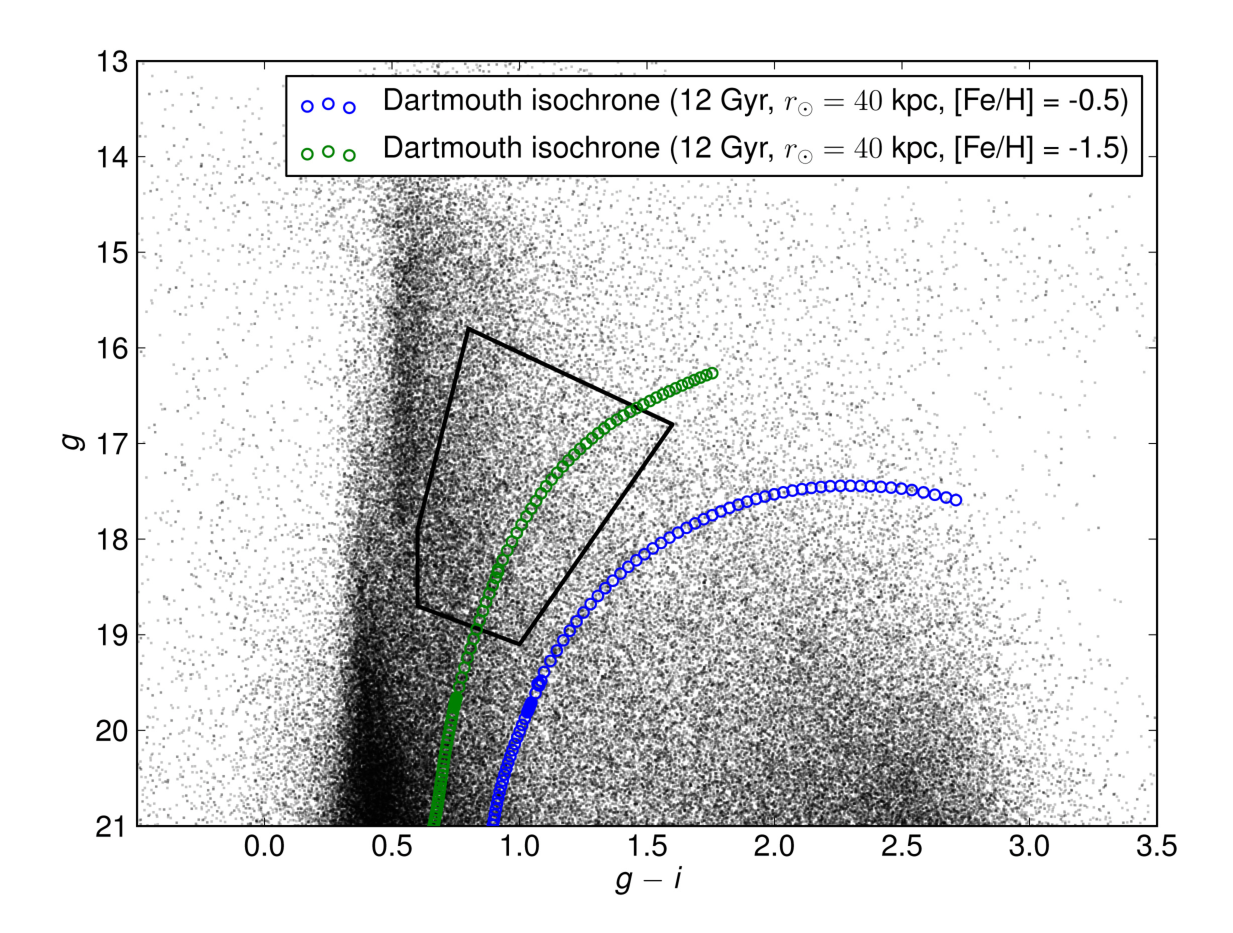
\includegraphics[width=\columnwidth]{./figures/cmd.eps}
	\caption{CMD of our observed regions from SDSS DR7, overlaid with the colour selection criterion used to target K-giants. Appropriate Dartmouth isochrones \citep{Dotter;et-al_2008} are shown for Sgr debris at a distance of $r_\odot =40$ kpc \citep{Belokurov;et-al_2006}}
	\label{fig:cmd-target-selection}
\end{figure}

\section{Observations}
\label{sec:observations}

Our targets were observed over two runs using AAOmega on the 3.9-m Anglo-Australian Telescope at Siding Springs Observatory in New South Wales, Australia. AAOmega is a double-beam, multi-object (392) fibre-fed spectrograph covering a two degree field of view. The targets were observed in normal visitor mode in April 2009. Throughout all observations, sufficient sky and guide fibres ($\sim30$ and 7-8 respectively) were allocated to ensure optimal sky subtraction and astrometry. In total 3,453 science targets were observed across 4 fields (Table \ref{tab:observations}). Multiple configurations were observed for most fields to permit measurements of bright ($i < 16$) and faint ($i > 16$) stars, as well as repeat observations on a subset of stars.

\begin{deluxetable}{cccc}
\tablecolumns{1}
\tablewidth{0pt}
\tabletypesize{\scriptsize}
\tablecaption{Observed fields\label{tab:observations}}
\tablehead{
	\colhead{Field} &
	\colhead{$\alpha$-center} &
	\colhead{$\delta$-center} &
	\colhead{Field} \\ 
	& (J2000.0) & (J2000.0) & Configurations
}
\startdata
A & 12 00 00 & $+00$ 00 00 & 1 \\ % & 188 \\ %180
B & 12 20 00 & $-01$ 00 00 & 2 \\ %& 673 \\ %185
C & 12 40 00 & $-02$ 00 00 & 3 \\ %& 870 \\ %190
D & 12 56 00 & $-02$ 42 00 & 6 \\ %& 1,722 %194
\enddata
\end{deluxetable}


The beam was split into the red and blue arms using the 5700 \AA{} dichroic. The 580V grating in the blue arm yields spectra between 370-580 nm, with a resolution of $R = 1300$. In the red arm we used the 1000I grating which spans the spectral range from 800-950 nm. This coverage includes the Ca II NIR Triplet (CaT), which is used for radial velocities and metallicities. To minimise scattered-light cross talk between fibres, science targets on each configuration were limited to 1.5 magnitudes in range. Globular clusters NGC 5024, 5053 and 5904 were observed as radial velocity and metallicity standards.

The data was reduced using the 2\textsc{DFDR}\footnote{http://www.aao.gov.au/AAO/2df/aaomega} pipeline. After being flat-fielded, the fibres were throughput calibrated and the sky spectrum was subtracted using the median of the dedicated sky fibres. Wavelength calibration was achieved from arc lamp exposures taken between each set of science fields. Multiple object frames were successively taken to assist with cosmic ray removal. %Three thirty-minute science exposures were taken for each faint field, and three twenty-five minute exposures for bright fields.

\section{Dwarf / Giant separation}
\label{sec:dwarf-giant-separation}

	When discussing our data with respect to stellar streams and substructures within the halo, we are referring only to K-type giants.  Dwarfs that fall within our apparent magnitude limit are not sufficiently distant to probe halo substructures. Our resolution is adequate such that the Mg I triplet lines can be individually measured and used to discriminate dwarfs. 	

%\begin{figure*}[t]
%	\includegraphics[width=\textwidth]{./figures/spectra.eps}
%	\caption{Blue arm spectra for a K-type giant (top) and dwarf (bottom) star, highlighting the difference in the gravity-sensitive Mg I triplet profiles at 5167.3, 5172.7 and 5183.6 \AA{}, and the typical fitting achieved.}
%	\label{fig:dwarf-giant-comparison}
%\end{figure*}

A grid of synthetic spectra has been generated to quantitively establish a giant/dwarf star separation criterion. The grid was generated using \citet{Castelli;Kurucz_2004} model atmospheres with MOOG\footnote{http://www.as.utexas.edu/$\sim$chris/moog.html} and the line list of \citet{Kurucz;Bell_1995}. Spectra was also generated using stellar parameters for the Sun and Arcturus. The strength of the Mg I lines were tuned to match both the Solar and Arcturus atlases of \citet{Hinkle;et-al_2003}. \citet{Girardi;et-al_2004} isochrones have been used to translate our de-reddened $g - i$ colour range to effective temperature. Reddening is accounted for using the maps of \citet{Schlegel;Finkbeiner;Davis_1998}. The corresponding effective temperature region ranges from 3900 to 5200 K, and is stepped at 25 K intervals. We have assumed typical K-type surface gravities of $\log{g} = 2$ for giants and $\log{g} = 4.5$ for dwarfs. Metallicities of [Fe/H] $= -0.5$, $-1.5$, and $-2.5$ were considered for both surface gravities.

All synthetic spectra was mapped onto the same wavelength space as our observations. Intensity was convolved with a Gaussian kernel of 3.03 \AA{} to match our observed resolution with the 580V grating. Mg I line strengths for our observations and synthetic spectra is shown against $g - i$ in Figure \ref{fig:dwarf-giant-separation}. As expected, there is an overlap of Mg I strengths between metal-rich ``giants'' ($\log{g} = 2$) and metal-poor ``dwarfs'' ($\log{g} = 4.5$). However, we do not expect metal-poor dwarfs to be a principle contaminant due to their intrinsically low luminosities and paucity.
\begin{figure}[h]
	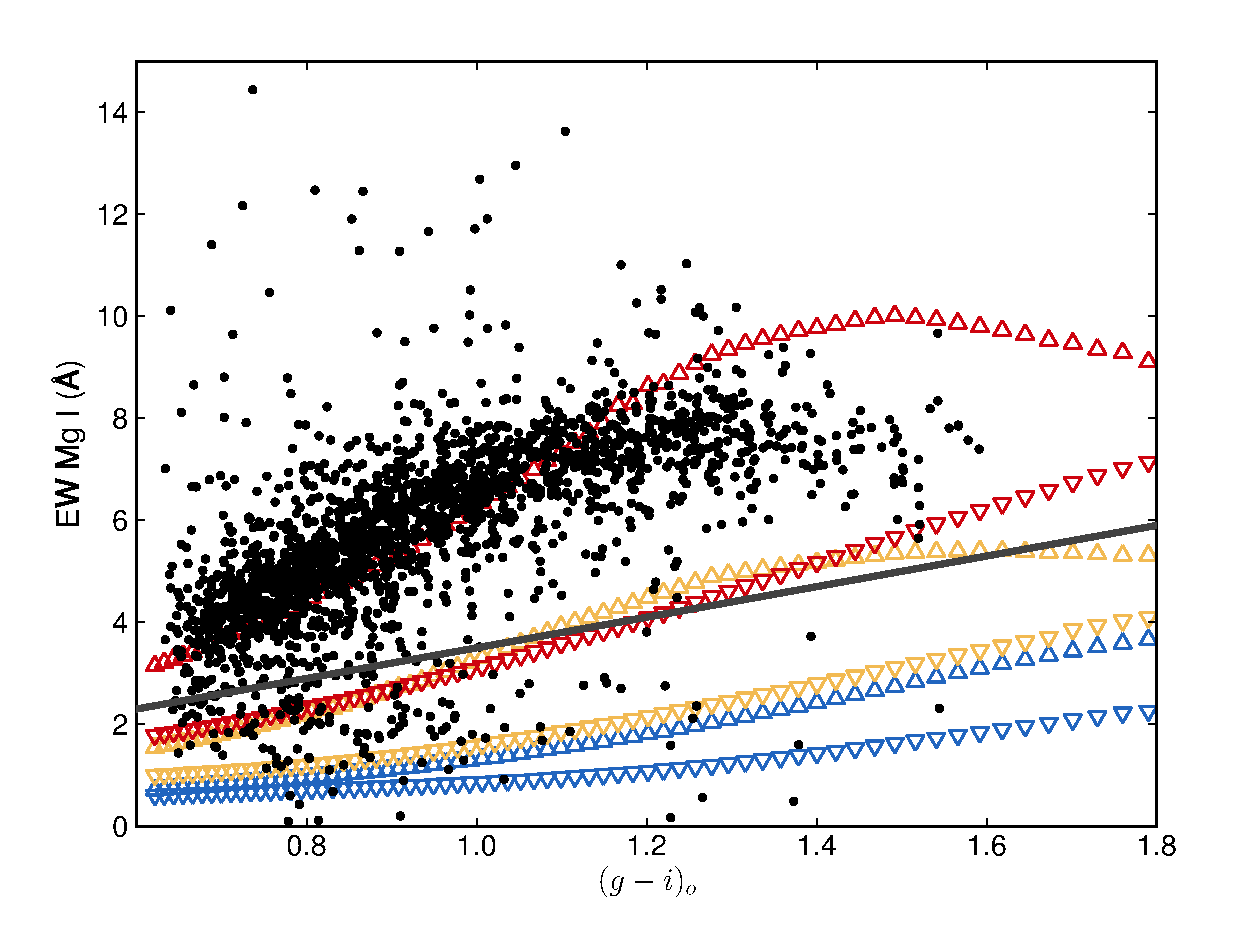
\includegraphics[width=\columnwidth]{./figures/dwarfgiants.eps}
	\caption{The sum of the Mg I triplet EWs for observations and synthetic spectra shown against the Sloan $g\,-\,i$ colour. Synthetic spectra is shown for $\log{g} = 2$ ($\bigtriangleup$) and $\log{g} = 4.5$ ($\bigtriangledown$), and points are coloured by metallicity. Our dwarf/giant separation line is shown (solid). }
	\label{fig:dwarf-giant-separation}
\end{figure}
 %The choice of separation criterion affects our dwarf contamination, and our giant recoverability. 
 Using our synthetic grid, we have varied the slope and offset of our separation line to assess the effectiveness in differentiating giants from dwarfs.  A linear rule has been adopted to differentiate the populations, which maximises giant recoverability with minimal contamination. Using the rule,
\begin{equation}
	EW_{Mg\,I} < 3(g-i) + 0.5
\end{equation}
\noindent we identify 185 giants in our observed fields. An analysis of our 185 giant candidates revealed three stars with high proper motions, all of which lay close to our dwarf/giant separation line. This suggests they are dwarfs, and have been excluded. Some possible giant targets were discarded due to insufficient S/N, or because the Mg I triplet fell on bad columns of the detector. All efforts were made to minimise these losses. The distilled giant sample size is 178.

	
\section{Radial Velocities}
\label{sec:kinematics}
%Their prominence allows us to determine accurate radial velocities even in noisy data. 

The Ca II triplet absorption lines at 8498.0, 8542.1 and 8662.1 \AA{}  have been used to measure radial velocities. These lines are strong, and easily identifiable in Red Giant Branch (RGB) stars even at low resolution.  Observed spectra have been cross-correlated with typical synthetic spectra of a K-giant ($T_{eff} = 4500$ K, $\log{g} = 2$, [Fe/H] $= -1.5$), and heliocentric corrections were made. Radial velocity measurements made on the standard stars in our globular clusters agree (within 3 km s$^{-1}$) with the catalogue of \citet{Harris_1996} (2011 edition). A number of our targets were observed on multiple fields, which allows us to calculate the internal measurement error. The differences between multiple measurements of the same target was calculated, and they form a half-normal distribution with a HWHM $= 3.58$ km s$^{-1}$. %This measurement includes velocity measurements of identified dwarfs, as we are focussed here on determining the systematic accuracy of our velocity measurements and not identifying substructures.

%\begin{figure}[h]
%	\includegraphics[width=\columnwidth]{./figures/vel_error.eps}
%	\caption{Internal radial velocity errors between multiple measurements. This sample includes all targets (dwarfs and giants) with sufficient S/N that were observed more than once.}
%	\label{fig:multiple-kinematics}
%\end{figure}
	
In order to compare our kinematic results in a homogenous manner, we have translated our heliocentric velocities to a galactocentric frame. We have adopted the circular velocity of the Local Standard of Rest (LSR) at the Sun as 220 km s$^{-1}$ \citep{Kerr;Lynden-Bell_1986} and accounted for the Sun's peculiar velocity to the LSR by using 16.5 km s$^{-1}$ towards $l = 53^\circ, b = 25^\circ$ \citep{Mihalas;Binney_1981}. The corrected line of sight velocity is then given by,
\begin{eqnarray}
	&V_{GSR} = & V_{OBS} + 220\sin{l}\cos{b} + 16.5  \\
	& 		 &\times[\sin{b}\sin{25} + \cos{b}\cos{25}\cos{(l - 53)}] \nonumber
\end{eqnarray}
\noindent where $V_{OBS}$ is the heliocentric corrected observed line of sight velocity. A caveat to this reference transformation is that other authors in the literature have used slightly different formulae to transpose their kinematics to a galactocentric frame. This will result in a systematic shift in velocities between authors of up to $\sim11$ km s$^{-1}$. 

\section{Metallicities}
\label{sec:metallicities}

We have ascertained metallicities for our giants using the strength of the Ca triplet lines. This technique was originally empirically described for individual stars in globular  clusters \citep{Armandroff;Da-Costa_1991}. A spectroscopic analysis using VLT/FLAMES observations of RGB stars from composite populations led \citet{Battaglia;et-al_2008} to conclude that a calibrated CaT-[Fe/H] relationship can be confidently used in composite stellar populations \citep[see also][]{Rutledge;Hesser;Stetson_1997, Starkenburg;et-al_2010}. The caveat to this technique is that a luminosity (specifically $V - V_{HB}$) is required for calibration, and we have to assume a $V_{HB}$ luminosity here. Johnson V-band magnitudes were calculated from SDSS \textit{ugriz} photometry using \citet{Jester;et-al_2005} transformations. The weaker third Ca triplet line is more susceptible to noise and residual sky-line contamination \citep{Tolstoy;et-al_2001,Battaglia;et-al_2008}. Consequently, the strongest two CaT lines (8542 and 8662\AA) have been used to form a reduced EW (W') such that,
\begin{comment}
%Nevertheless the CaT-[Fe/H] relationship is strong for RGB stars in composite populations within the range $-2.5 < \mbox{[Fe/H]} < -0.5$.

%However, a systematic trend in this high resolution spectra was found where metallicity is overestimated by $\sim0.1$ dex at low metallicities ($\mbox{[Fe/H]} < -2.2$) and underestimated by $\sim0.1-0.2$ dex at higher metallicities ($\mbox{[Fe/H]} > -1.2$) using this calibration. \citet{Battaglia;et-al_2008} indicate higher Ca abundances may affect the CaT equivalent width sufficiently to cause this trend, although [Fe/H] is the certain dominant factor contributing to the CaT line strength. 	

%The [Ca/H] - [Fe/H] association is linear, although this technique is only applicable for stars brighter than the horizontal branch ($V - V_{HB} > 0$). Transformations from SDSS $ugriz$ photometry to $UBVR_{C}I_{C}$ has been performed using the transformation equations in \citet{Jester;et-al_2005}. Photometric errors (including those from transformations) are propagated to our reported metallicity errors.

%The sum of the CaT EW is scaled to form a 'reduced EW' (W'). There is some discussion in which combination of the three CaT lines should be used. In this work we have taken the total equivalent width as the sum of the two stronger Ca lines ($\lambda_{8542}$, $\lambda_{8662}$). The weakest Ca line is usually the most unreliable when calculating equivalent widths due to noise and the possibility of residual sky-line contamination. Moreover, following a comparison of scaling relations between CaT and [Fe/H], \citet{Battaglia;et-al_2008} found using only the two strongest lines (as \citet{Tolstoy;et-al_2001} had done) was the most robust. As such, we have adopted the best-fitting relationship found by \citet{Battaglia;et-al_2008} for this work. The reduced EW is calculable by
\end{comment}
\begin{eqnarray}
	\textstyle\sum{W}\, &=& EW_{8542} + EW_{8662} \\
	W' &=&\textstyle\sum{W} + 0.64\left(\pm 0.02\right)\left(V-V_{HB}\right)
\end{eqnarray}
\noindent and the metallicity linearly varies with W' where,
\begin{equation}
	\mbox{[Fe/H]}_{\mbox{\small{CaT}}} = (-2.81\pm0.16) + (0.44\pm0.04) W'
	\label{eq:feh-cat}
\end{equation}

Using this calibration, our globular cluster standard stars (with known $V_{HB}$ magnitudes) have metallicities that match well with the \citet{Harris_1996} catalogue (2011 edition). Only K-giants within the valid calibration range ($0 > V-V_{HB} > -3$) were considered for metallicities. We assume that we have two dominant substructures present in our observations; the leading arm of Sagittarius and the Virgo Over-Density (see \S\ref{sec:substructure-identification}). The Sagittarius stream dominates our negative $V_{GSR}$ population, and our positive kinematic space is primarily comprised of VOD members. As such we have separated our population at $V_{GSR} = 0$ km s${-1}$ into two samples with assumed $V_{HB}$ magnitudes. Although this introduces a (known) systemic effect, it is a required assumption to estimate the metallicity distribution of each population.

The horizontal branch magnitude assumed for the VSS/VOD has been ascertained from previous RR Lyrae studies. As RR Lyraes sit on the horizontal branch, the $V_{HB}$ is taken as the V-band median of four \citet{Prior;et-al_2009a} and three  \citet{Duffau;et-al_2006} VSS members to yield $\langle{}V\rangle{} = 17.09$. This combined value precisely matches the mean solely reported by \citet{Duffau;et-al_2006}. In our K-giant sample with positive galactocentric velocities, we assume $V_{HB} = 17.09$ which implies these stars are at a distance of $\sim20$ kpc.

\begin{comment}
%When applying this technique to our K-giants, the difficulty is that $V_{HB}$ is not easily defined. The horizontal branch magnitude varies between stellar systems, and is dependent on the heliocentric distance to, and morphology of, the stellar environment.

%Observations here include a composite population. Some stars are members of the Sgr leading arm, others are members of the VOD/VSS (see \S\ref{sec:substructure-identification}), all superimposed upon a background of halo stars. We can identify some substructures kinematically, but we cannot differentiate halo stars within those velocity bins. However in our observed region there are known dominant structures. The Sagittarius stream dominates our negative $V_{GSR}$ population, and our positive kinematic space is largely comprised of members from the VOD (see \S\ref{sec:substructure-identification}). As such we have separated our population at $V_{GSR} = 0$ into two samples to ascertain $V_{HB}$ for the two most dominant populations; Sgr and the VOD. Although this technique introduces a (known) systemic effect, it is the most useful way to estimate the metallicity distribution of each population.
\end{comment}

As the distance to the Sgr debris varies greatly throughout the halo, the horizontal branch magnitude varies with the position along the stream. 
Through CMD comparisons with the Sgr core \citep{Bellazzini;et-al_2006}, \citet{Belokurov;et-al_2006} determined distances along the two branches of the Sgr bifurcation.  Revised distance measurements by \citet{Siegel;et-al_2007} (as tabulated in Table 1 of LM10) have been crucial in constraining dark halo models. Our observations lay on the edge of Branch A (Figure \ref{fig:sgr-field-of-streams}).

We have assumed distances to these stars by interpolating their position along a cubic spline fitted to published distances \citep{Siegel;et-al_2007}. Recent distance measurements of the stream by \citet{Ruhland;et-al_2011} match the stream distances used here within the uncertainties. The horizontal branch magnitude $V_{HB}$ is calculated using this assumed distance and the known luminosity of RR Lyrae stars \citep[$M_V = +0.69;$][]{Tsujimoto;et-al_1998}. Typical $V_{HB}$ magnitude derived for the Sgr members is $18.7$, at a distance of $\sim{}41$ kpc. Reddening is accounted for using the \citet{Schlegel;Finkbeiner;Davis_1998} maps. Uncertainties in distance are not interpolated; they are taken as the largest published uncertainty of the closest neighbouring data points, and this is propagated through to our reported metallicity uncertainties. 

\begin{comment}
The horizontal branch magnitude for the Sgr debris varies with age and distance. \citet{Belokurov;et-al_2006} determined distances along the two branches of the Sgr bifurcation using a colour-magnitude comparison with the Sgr main body \citep{Bellazzini;et-al_2006}. After being scaled for a revised distance modulus to the Sgr core \citep[$(m-M)_{0} = 17.27;$][]{Siegel;et-al_2007}, these distance measurements were used to constrain the more recent tri-axial halo simulation by LM10.  We can use these observed distances (as tabulated in Table 1 of LM10) and the known absolute magnitude of RR Lyrae stars \citep[$M_V = +0.69;$][]{Tsujimoto;et-al_1998} to calculate the horizontal branch magnitude for each position of the Sgr stream. Reddening is accounted for each star using the maps of \citet{Schlegel;Finkbeiner;Davis_1998} and is scaled to the V-band with $A/E(B-V) = 3.240$. A spline is fitted to the tabulated right ascension and distance measurements, and the distance to each star is found by evaluating the right ascension of each star along the spline. Distance to the branch does not vary significantly with declination. The distance error is taken as the largest error from the two neighbouring distance measurements.
%Distance errors are also propagated through to our reported metallicity error, which is at most $\sim 0.16$ dex. 
\end{comment}

\section{Discussion}
\label{sec:discussion}
	
		%Along our line of sight, the spatial region examined in this paper incorporates the superposition of multiple substructures, some of which may be inter-related. To facilitate a logical flow of discussion, these substructures are identified first and discussed separately. 	
		
	\subsection{Substructure Identification}
	\label{sec:substructure-identification}
		
A significant kinematic deviation from a canonical halo population signifies a co-moving group. There are multiple substructures along our line-of-sight. These features are identified first and discussed separately. We have represented our galactocentric velocities with a generalised histogram (Figure \ref{fig:velocity-histogram}) to quantitatively compare the observed stellar kinematics against the hypothesis that the parent distribution ca be described by a canonical halo ($\mu = 0$ km s$^{-1}$, $\sigma = 101.6$ km s$^{-1}$ \citep{Sirko;et-al_2004}).

	\begin{figure}[h!]
		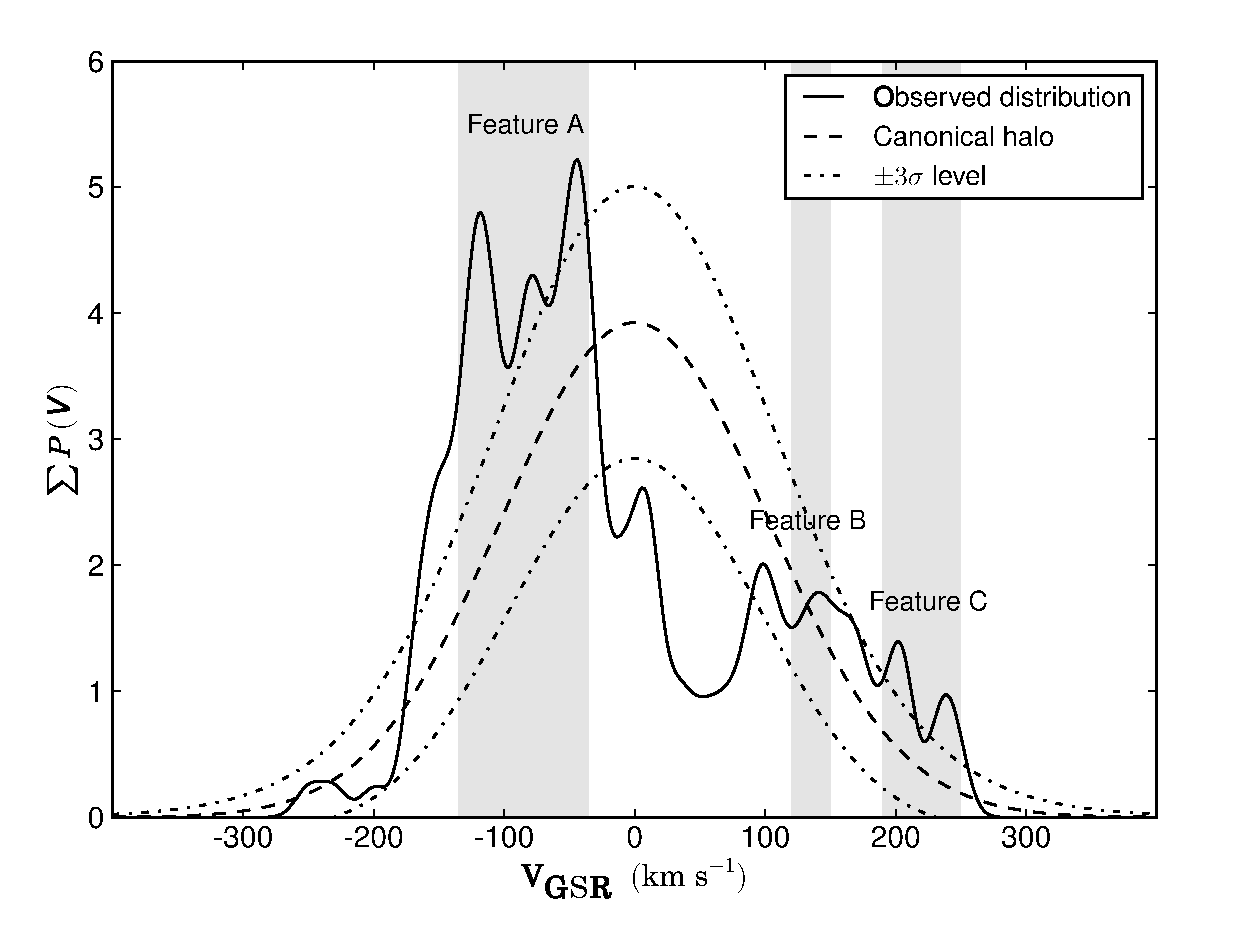
\includegraphics[width=\columnwidth]{./figures/velocity-halo.eps}
		\caption{Generalised histogram of $V_{GSR}$ for our 178 K-type giants, highlighting their significance against a canonical halo population. The Gaussian is normalised such that the integral equals the number of observed stars excluding those outside a 2.5-$\sigma$ excess. Significant ($>3\sigma$) kinematic deviations from the smooth distribution are appropriately grouped and labelled.}
		\label{fig:velocity-histogram}
	\end{figure}
	
The generalised histogram represents each data point with a Gaussian kernel of an equal bandwidth (deviation). As our internal kinematic errors between multiple measurements summate to a half-normal distribution with a FWHM of 7.16 km s$^{-1}$, we have opted for a bandwidth value of 10 km s$^{-1}$ the generalised histogram in Figure \ref{fig:velocity-histogram} to avoid under-smoothing.

	\begin{figure}[h!]
		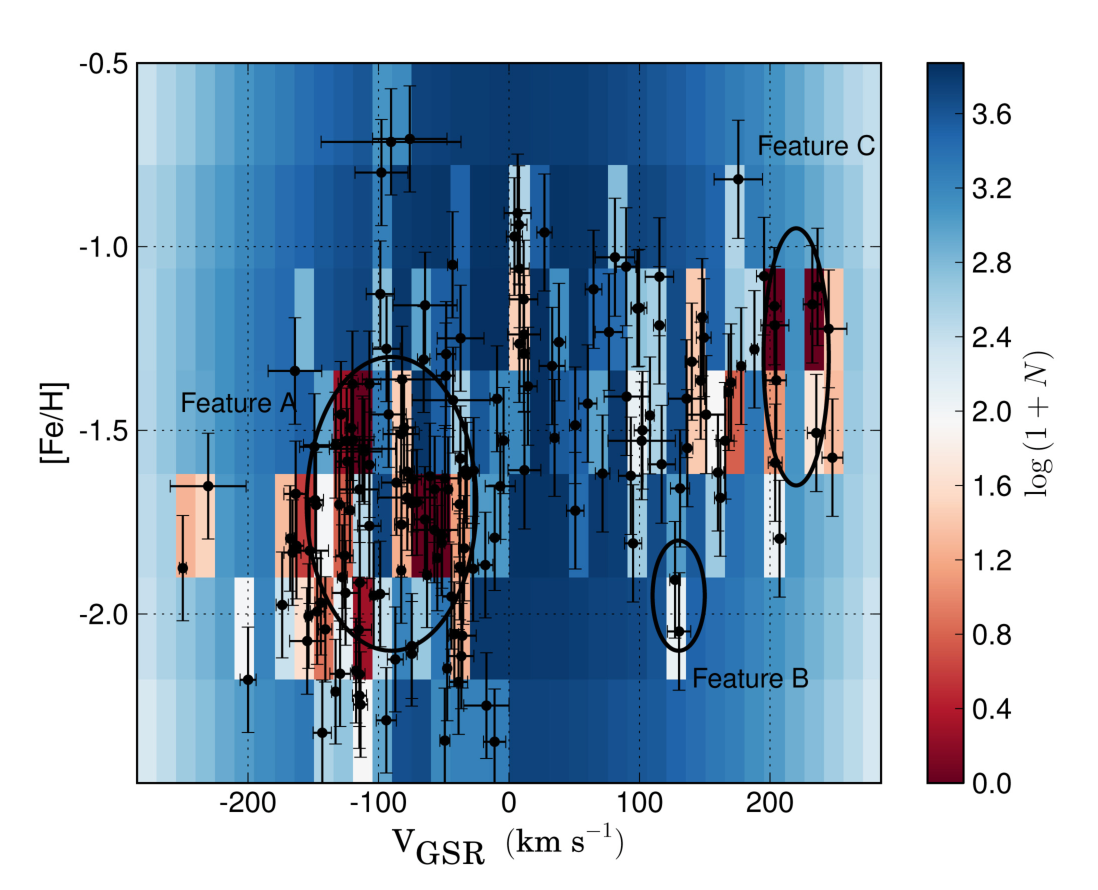
\includegraphics[width=\columnwidth]{./figures/montecarlo.eps}
		\caption{Monte-Carlo simulation results illustrating the number of times simulations could reproduce our observed data in the equivalent multi-dimensional bin. Significant features discussed in the text are labelled.}
		%\caption{Results from our 10,000 binned kinematic and chemical Monte-Carlo simulations, overlaid with our observed K-giant sample properties. Each bin is coloured by the number of times Monte-Carlo simulations reproduced at least the same number of observed stars in that bin. Red bins indicate particularly rare clumps, and blue bins demonstrate common samples.}
		\label{fig:monte-carlo}
	\end{figure}
%We have looked at stars in our dataset with repeated observations to gain an approximation for the bandwidth selection.
% Their statistical significance is determined by a comparison to a canonical halo population \citep[$\mu = 0$ km s$^{-1}, \sigma = 101.6$ km s$^{-1}$][]{Sirko;et-al_2004}.

	\begin{figure*}[t!]
		%\plottwo{./figures/belokurov2006.eps}{./figures/belokurov2006.eps} %#todo - bw/color + newline for caption
		\includegraphics[width=\textwidth]{./figures/belokurov2006.eps}
		\caption{Observed fields are outlined upon a panoramic view of the Sgr stream, to demonstrate our field locations in context with the Sagittarius stream. This plot is an adaptation of Figure 2 in \citet{Belokurov;et-al_2006}, which uses the 2MASS M-giant sample of \citet{Majewski;et-al_2003}.}
		\label{fig:sgr-field-of-streams}
	\end{figure*}
	
	The most significant ($>3\sigma$) kinematic peaks have been labeled Features A, B, and C. Features A and C are our most significant structures, and the importance of Feature B becomes more evident through Monte-Carlo simulations. Velocities and metallicities of our K-giants have been binned into grid blocks of 15 km s$^{-1}$ and 0.3 dex \--- roughly twice the error in each dimension. A population of 178 stars were randomly drawn from a simulated halo with canonical kinematics. Metallicities were randomly assigned using the observed halo Metallicity Distribution Function (MDF) of \citet{Ryan;Norris_1991}. Each simulated population was binned identically to our observed sample. Simulation grid blocks with counts equal to or exceeding stars in our equivalent observed grid block were noted, and summed after 10,000 simulations. Results from our Monte-Carlo simulations are illustrated in Figure \ref{fig:monte-carlo}. These were consistently significant when the grid was midpoint offset in both dimensions, except for the grid-block centered at $\sim185$ km s$^{-1}$ and $\sim-1.4$ dex, which has consequently been left unlabelled.
	
	 Substructure becomes statistically significant when the observed grid blocks are rarely replicated in Monte-Carlo simulations. Specifically, the number of members in Feature A of Figure \ref{fig:velocity-histogram} was never reproduced in some grid bins. This feature is well in excess of the halo and has a wide spread in kinematics. \citet{Chou;et-al_2007} mapped the Sgr debris across the sky using K/M-giants and found galactocentric velocity signatures between $-205$ km s$^{-1}$ to $-31$ km s$^{-1}$ in this region. As such we attribute this wide, significant kinematic peak as the leading arm of the Sagittarius tidal tail. Feature A is discussed in the next section. Another feature where grid blocks were never reproduced in our simulations was Feature C. This feature may also be attributed to Sgr debris and is discussed further in \S\ref{sec:feature-c}.
	 	
	 The clump of stars in the velocity bin centered on $V_{GSR} \approx 130$ km s$^{-1}$ and [Fe/H] $\approx -2$ was replicated only $\sim1$\% in 10,000 simulations. We attribute these members to the Virgo Stellar Stream. These members are coincident in spatial position, velocity, and metallicity with previously reported values of the VSS obtained by F turnoff/BHB stars \citep{Newberg;et-al_2007} and RR Lyrae stars \citep{Prior;et-al_2009a}. Feature B is discussed in \S\ref{sec:the-vss}.


	\subsection{Feature A \--- Sagittarius Debris}
	\label{sec:sgr-debris}


		
	The bounds of our observed region are overlaid upon a panoramic projection of the Sagittarius stream, and the  ``Field of Streams''  \citep{Belokurov;et-al_2006} in Figure \ref{fig:sgr-field-of-streams}. This is a crowded region of globular clusters, substructures and overlapping stellar streams, primarily populated by the Sagittarius Northern leading arm. Simply from a spatial perspective, we expect the Sgr debris to dominate our data. Although the VOD is present, it is much more diffuse. 
\begin{comment}
%It is useful to see how our fields spatially overlap with the Sgr stream. 
	%\textit{N}-body models of the Sgr stream suggest highly negative velocities in this region (LJM05, LM10). This has led several authors who have observed negative kinematic peaks in nearby fields \citep{Yanny;et-al_2009, Prior;et-al_2009b}, to attribute these as members of Sagittarius as we have here.
	
	%The bifurcation in Sagittarius \citep{Belokurov;et-al_2006} is evident here, and our observed fields overlap with the the lower declination Branch A.
	%The consequential tidal tails from the Sgr-Milky Way interaction has been modelled by many groups \citep[e.g. ][]{Helmi_2004, Law;et-al_2005, Law;Majewski_2010}. 
\end{comment}

	\subsubsection{Comparing Sagittarius Debris to Dark Matter Halo Models}	

	In order to investigate the spatial coverage and kinematics of our Sagittarius members, we have compared our giants with the constant flattening spheroidal models of LJM05 and the more recent tri-axial model of LM10. The simulated data output from these is readily available online\footnote{http://www.astro.virginia.edu/$\sim$srm4n/Sgr/}, and their released models have the best-fitting parameters for each dark halo shape (prolate, spherical, oblate and tri-axial).  These are the only simulations available which make use of an all-sky data set; the 2MASS M-giant sample. We have not considered particles farther than 60 kpc to match realistic observation limitations. For comprehensive details of the simulations the reader is referred to the papers of \citet{Law;et-al_2005} and \citet{Law;Majewski_2010}. 
%Simulations are matched to the 2MASS M-giant sample, which provides an all-sky view of the Sgr stream. %\citet{Law;et-al_2005} describe the Milky Way as a smooth, rigid potential and represent Sgr with $10^5$ self-gravitating particles. The Galactic potential is represented with three primary components; a \citet{Miyamoto;Nagai_1975} disk, a Hernquist spheroid and a logarithmic halo. The models of LJM05 have a constant degree of flattening, $q$, whereas the more recent LM10 tri-axial model has a minor/major axis ratio $(c/a)_\Phi = 0.72$ and an intermediate axis ratio $(b/a)_\Phi = 0.99$ at radii $20 < r < 60$ kpc.  Their simulations adopt a spherical heliocentric coordinate system ($\Lambda_\odot, B_\odot$) where the longitudinal axis $\Lambda_\odot = 0^\circ$ at the Sgr core, and $B_\odot$ represents the best fitting great circle of the Sgr debris. For comprehensive details of the simulations the reader is referred to the papers of \citet{Law;et-al_2005} and \citet{Law;Majewski_2010}. The spatial distribution of the simulated Sgr tidal tails are illustrated in Figure \ref{fig:law-spatial}, which shows the simulated particles from the LJM05 and LM10 models, and our observed fields. To match realistic observation limitations we have not considered particles farther than 60 kpc.
		
	\begin{figure}[t!]
		\includegraphics[width=\columnwidth]{./figures/lawspatial.eps}
		%\plottwo{./figures/law_spatial_copy.eps}{./figures/law_spatial_copy.eps} %#todo - b/w version
		\caption{Our fields and observed bounds are shown with the simulated particles from multiple \textit{N}-body simulations by LJM05 and LM10. These particles are distance restricted (up to 60 kpc), and colour-coded by their peri-centric passage following the same convention by \citet{Law;Majewski_2010} (orange;most recent passage, magenta; previous passage, cyan; oldest observable passage).}
		\label{fig:law-spatial}
	\end{figure}
%To evaluate how well models predict the position and kinematics of the Sgr debris, we require either a large set of accurate stellar kinematics and distances, or targeted regions of the stream where a change in the shape of the dark halo results in significantly different simulated positions and kinematics. The latter is particularly the case for our fields . 	

	The Northern leading arm of Sgr is particularly sensitive both kinematically and spatially to the shape of the Milky Way dark halo (Figure \ref{fig:law-spatial}). Most models predict the Sgr stream to pass directly through our fields, whereas the prolate model predicts the edge of the stream near this region and no particles directly in our fields. Spatially, the prolate model predicts the Sgr stream to pass much lower in $B_\odot$ than our observed fields. When we extend a rectangle bounded by the edges of our fields (as per the zoomed insets in Figure \ref{fig:law-spatial}) a mere two particles are predicted. If this prolate halo model is a true representation of the Sgr debris, this does not exclude the potential of finding some Sgr debris in our fields. However, it does imply that if the LJM05 prolate model is an accurate representation of the dark halo then Sgr would not be the dominant population, contrary to our preferred interpretation of the observations.
	
	In comparison the tri-axial, spherical and oblate models predict varying debris from previous peri-centric passages in our fields. A kinematic comparison against our observations is necessary to evaluate model predictions. As the prolate model has only two simulated particles within our extended bounds there is no qualitative kinematic comparison to be made for this model, and as such the prolate model is excluded from further kinematic analysis.

	\begin{figure*}[t!]
		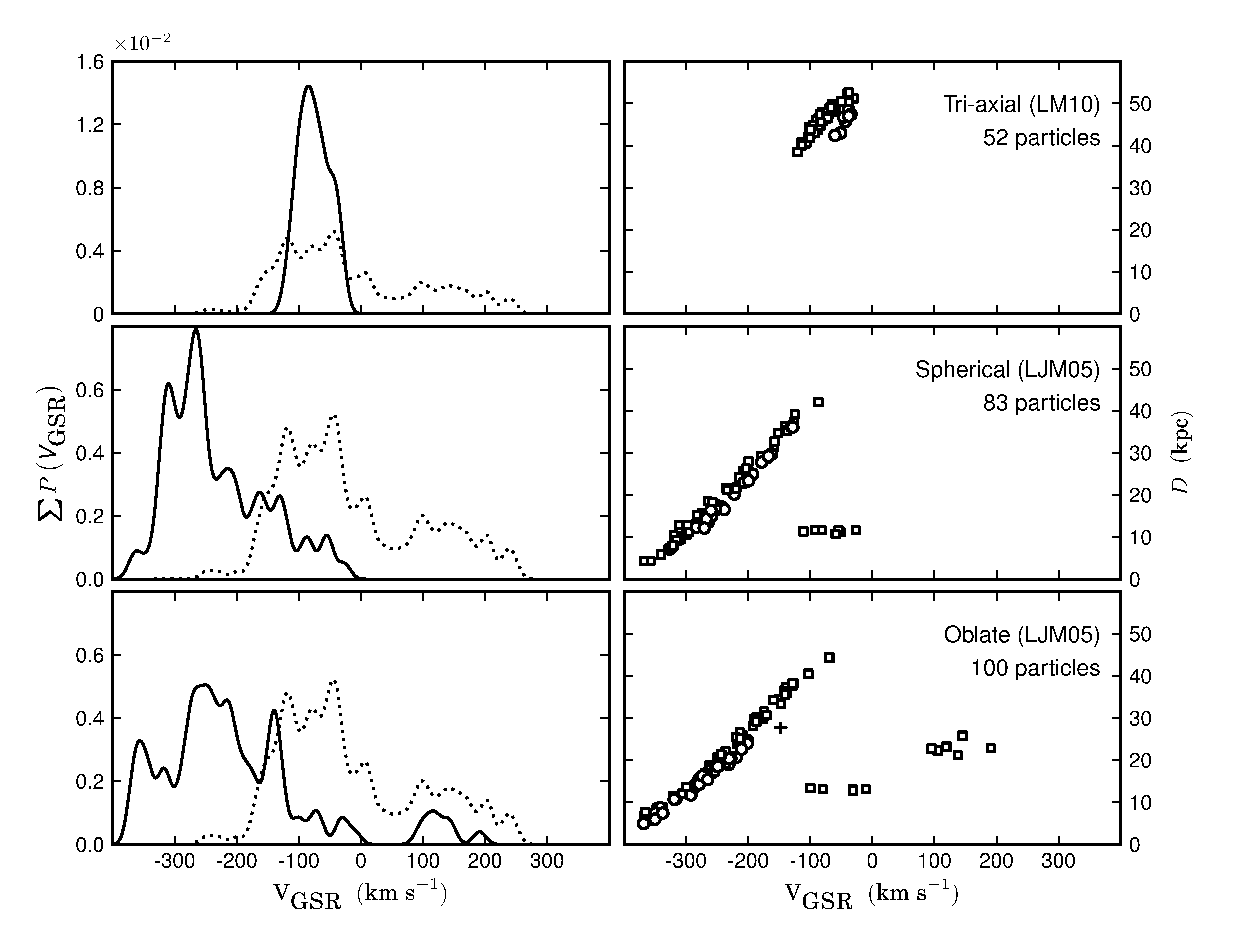
\includegraphics[width=\textwidth]{./figures/lawvelcompare-bw.eps}
		\caption{A generalised histogram (left) of the galactocentric rest frame velocities in our sample (dotted line) compared to the velocities (solid line) from the \textit{N}-body models of LJM05, LM10 of particles within the same spatial coverage and distance range (up to $r_\odot \sim 60$ kpc) of our observed sample. Heliocentric distances for particles used to generate each velocity histogram are shown on the right. Particles are marked by their recency of passage. A plus ($+$) denotes debris from the current peri-centric passage by Sgr, circles ($\circ$) mark the previous passage, and squares ($\square$) represent debris from two previous passages. The prolate model from LJM05 is not considered in this plot (see text).}
		\label{fig:law-vel-compare}
	\end{figure*}
	
	The number of predicted particles observable differs between models. Consequently the kinematics for each model have been represented as a generalised histogram (Figure \ref{fig:law-vel-compare}). For consistency all simulation output and observed data has been convolved with a Gaussian kernel of 10 km s$^{-1}$; the bandwidth used for the previous generalised histogram in Figure \ref{fig:velocity-histogram}. Predicted distances and peri-centric ages are shown, demonstrating that debris from multiple passages are predicted along the line of sight. A much tighter velocity sequence is predicted here by the tri-axial model than the constant flattening models. This is because the tri-axial model predicts a pericenter almost precisely in our observable region, whereas the spherical and oblate models forecast a large wrap along the line of sight, resulting in a wide spread of distances and velocities.
	
	 %A generalised histogram is an effective method to evaluate the model predictions, because the size the overall distribution is scaled such that the integral of each distribution is unity. Therefore populations of different sizes (i.e. our observed sample and the varying size of each simulation output) are scaled appropriately so we can compare the kinematic signatures. One caveat of this technique is that the relative size of each sample must be acknowledged when evaluating the predictions made by a model. A narrow distribution \--- which may perfectly match the observed data \--- may simply be a consequence of an extremely small sample size, yielding an ineffective comparison. Indeed if we included a comparison with the prolate model the entire distribution may appear to represent the observed data closely in a qualitative sense, however that distribution would be composed from a mere two simulated particles.
%One caveat for generalised histograms is that a narrow distribution (which may perfectly match observations) may simply be a consequence of a small number of predicted particles, yielding an ineffective comparison. With this caveat in mind we have shown the simulated particle distances in Figure \ref{fig:law-vel-compare}. In this region there is debris from multiple passages predicted along the line of sight. Particles have been marked by their recency of peri-centric passage. Distinguishing particles by their peri-centric age allows us to qualitatively differentiate relative kinematic contributions of the stream. In all three models, the Northern arm is clearly distinguishable, albeit the tri-axial model has a much tighter sequence in velocity. This is attributed to the position of the predicted pericenter. The tri-axial model predicts a pericenter almost precisely where our fields were observed, whereas the spherical and oblate model predict a large wrap of the stream along the line of sight, resulting in a large spread in kinematics and heliocentric distances.

	Predicted distances are consistent with what we would expect from our observations. The median luminosities of our giants is $g\sim17.5$, so for the tri-axial model particles at $45$ kpc this corresponds to an absolute magnitude of $M_g\sim-0.8$; quite reasonable for a K-giant. Similarly for the spherical and oblate models, typical distances of $\sim25$ kpc will yield luminosities of $M_g\sim+0.5$ which is also reasonable.  
	
	The spherical and oblate models also predict close-by debris with extremely negative galactocentric velocities. This signature is not represented in our data. Much closer K-giants are less likely to be identified given our luminosity range, although these early K-giants are much more numerous, so this is unlikely to explain our lack of highly negative kinematics.  The lowest observed velocity is $\sim{}-250$ km s$^{-1}$ and we have only two observations less than $V_{GSR} < -200$ km s$^{-1}$. In contrast, the spherical/oblate models predict velocities well below $V_{GSR} < -300$ km s$^{-1}$. These predicted highly negative  velocities were also not found in Sgr RR Lyrae observations taken by \citet{Prior;et-al_2009b}. If the dark matter potential is well-represented by either an oblate or spherical halo, then this discrepancy must be reconciled. 
	
	The oblate and spherical model also illustrate a similar signature at $r_\odot \sim$12 kpc, with particle velocities ranging between $-100 < V_{GSR} < 0$ km s$^{-1}$. This is the edge of a predicted crossing-point between different wraps of the stream, which occurs at $\sim12$ kpc. These particles (and the positive kinematic signature around $\sim$20 kpc in the oblate model), are relatively minor signatures when compared to the Northern arm feature. If these signatures are present in our observed fields, their relatively low density compared to the northern arm feature would prevent them from appearing as significant. %Therefore, we cannot use the edge particles of these nearby simulated wraps to discern substantial information regarding the dark halo of the Milky Way.

	Although the predicted velocity distribution is narrower than what we observe, the LM10 tri-axial dark halo model best fits our observations. The observed sample broadens most prominently towards more negative galactocentric velocities at $\sim-200$ km s$^{-1}$, still well higher than oblate/spherical predictions. Halo contamination at highly negative velocities is likely to be small. One reconciliation for this tri-axial model/observed kinematic discrepancy may lie in the workings of the tri-axial model itself. Unlike other models considered, the tri-axial model does not reproduce the observed bifurcation in the Sgr stream \citep{Belokurov;et-al_2006}. Although observationally untested, it is reasonable to suggest a kinematic disruption may result from the bifurcation. Such an effect would result in a broader kinematic distribution especially at the stream edges, precisely as seen in our data.
\begin{comment}		
	Although the debris kinematics may plausibly match our data, the tri-axial particles are predicted to be farther away than other model predictions. The tri-axial distribution is much narrower than our observed sample. Halo contamination in this distribution is likely to be small. The profile broadening in our sample extends most prominently at highly negative galactocentric velocities ($\sim-200$ km s$^{-1}$). Given any Gaussian-like population with a mean near zero, we would expect less halo members at high galactocentric velocities \--- positive or negative. One reconciliation for this profile discrepancy may lie in the workings of the tri-axial model itself. Unlike the other models compared here from LJM05, the tri-axial model does not reproduce the bifurcation observed in the Sgr stream \citep{Belokurov;et-al_2006}. Studies prior to the model development suggested the bifurcation may result from the progenitor internal dynamics, and not primarily consequential from the shape of the Milky Way dark halo \citep{Fellhauer;et-al_2006, Penarrubia;et-al_2010}. However a later study by \citet{Penarrubia;et-al_2011} found no evidence for internal rotation in the remnant core sufficient to produce the bifurcation.
	
	A comparative targeted study along each branch is necessary to discern a kinematic disruption. Our observed region lies on the lower declination Branch A. Given that, the spread in velocity associated with a bifurcation would be observed.

	The lack of bifurcation treatment in the LM10 model may explain the particularly narrow distribution predicted. Other groups have observed the spatial disruption caused by the bifurcation, however whether a kinematic variation exists between branches is observationally untested. Given the kinematic interactions within the progenitor, and the gravitational influence of the halo, it is reasonable to suggest a kinematic disruption may consequent from the bifurcation.  Such an effect may result in a wider kinematic distribution, precisely as seen in our data. 
	% If these distance predictions are accurate they would likely be outside our observable range. Clearly more detailed investigation is required.
\end{comment}
	
	There is further work required through observations and simulations to reconcile kinematic discrepancies. Typical examinations of the leading arm debris usually favour prolate halos and evidence along the trailing arm typically favours oblate halos \citep{Helmi_2004, Martinez-Delgado;et-al_2004, Law;et-al_2005}. Kinematic predictions of the LM10 tri-axial model reasonably match our observations, whereas the prolate model has been excluded as significant debris is not predicted in this edge of the stream. These observations along the Northern leading arm are the first which are not reproducible with the current prolate model of LJM05, contrary to previous groups who have surveyed closer to the leading arm debris.

	\subsubsection{A Metal-Poor Population Uncovered in Sagittarius Debris}
	\label{sec:sgr-metal-poor}

	%The Sgr progenitor is a composite stellar population with a radial abundance declivity. As the host circles the Milky Way the older, more metal-poor stars are preferentially stripped from the progenitor \citep{Piatek;Pryor_1995}. 
	%While the core hosts the more metal-rich members \citep{Bonifacio;et-al_2004, Monaco;et-al_2005}, the most ancient wraps of the stream comprises the more metal-poor members \citep{Chou;et-al_2007}. 
		
	Many groups have found the population of the Sgr core to possess a mean [Fe/H] $\sim -0.5$ dex \citep{Cacciari;et-al_2002, Bonifacio;et-al_2004, Monaco;et-al_2005}. As the host circles the Milky Way the older, more metal-poor stars are preferentially stripped from the progenitor, creating a metallicity gradient along the stream \citep{Chou;et-al_2007, Keller;Yong;Da_Costa_2010}. In this region of the stream, very few Sgr member metallicies have been reported. \citet{Vivas;et-al_2005} found a mean metallicity of $\langle$[Fe/H]$\rangle = -1.77$ from spectra of 16 RR Lyraes along a nearby region of the Sgr leading arm. Similarly, \citet{Prior;et-al_2009b} found $\langle$[Fe/H]$\rangle = -1.79 \pm 0.08$ for 21 type \textit{ab} RR Lyrae stars in the region. This is somewhat expected since only the oldest, most metal-poor stars can form RR Lyraes. 
	
	Investigating the MDF of the Sgr debris requires an unbiased sample. Generally K-giants are excellent stellar candidates for such investigations as all stars go through this evolutionary phase whereas M-giants are consistently metal-rich. If we apply the metallicity gradient found by \citet[][from M-giants]{Keller;Yong;Da_Costa_2010} to these observed K-giants, we would expect an abundance mean near $\sim{}-1.2$ dex in this observed region. The metallicity distribution for our negative $V_{GSR}$ sample is shown in Figure \ref{fig:sgr-metallicity-hist}, and illustrates a metal-poor population. The mean of our distribution is $\langle$[Fe/H]$\rangle = -1.7\,\pm\,0.3$ dex. If we include only the stars attributed to Feature A (Sgr debris) this value increases by only 0.04 dex, well within observational uncertainties. As a comparison, in a sample of metal-rich biased M-giants from the 2MASS data \citet{Chou;et-al_2007} found a mean metallicity of $\langle$[Fe/H]$\rangle = -0.72$ dex for their best subsample in the Northern leading arm of Sgr.
	
	\begin{figure}[h]
		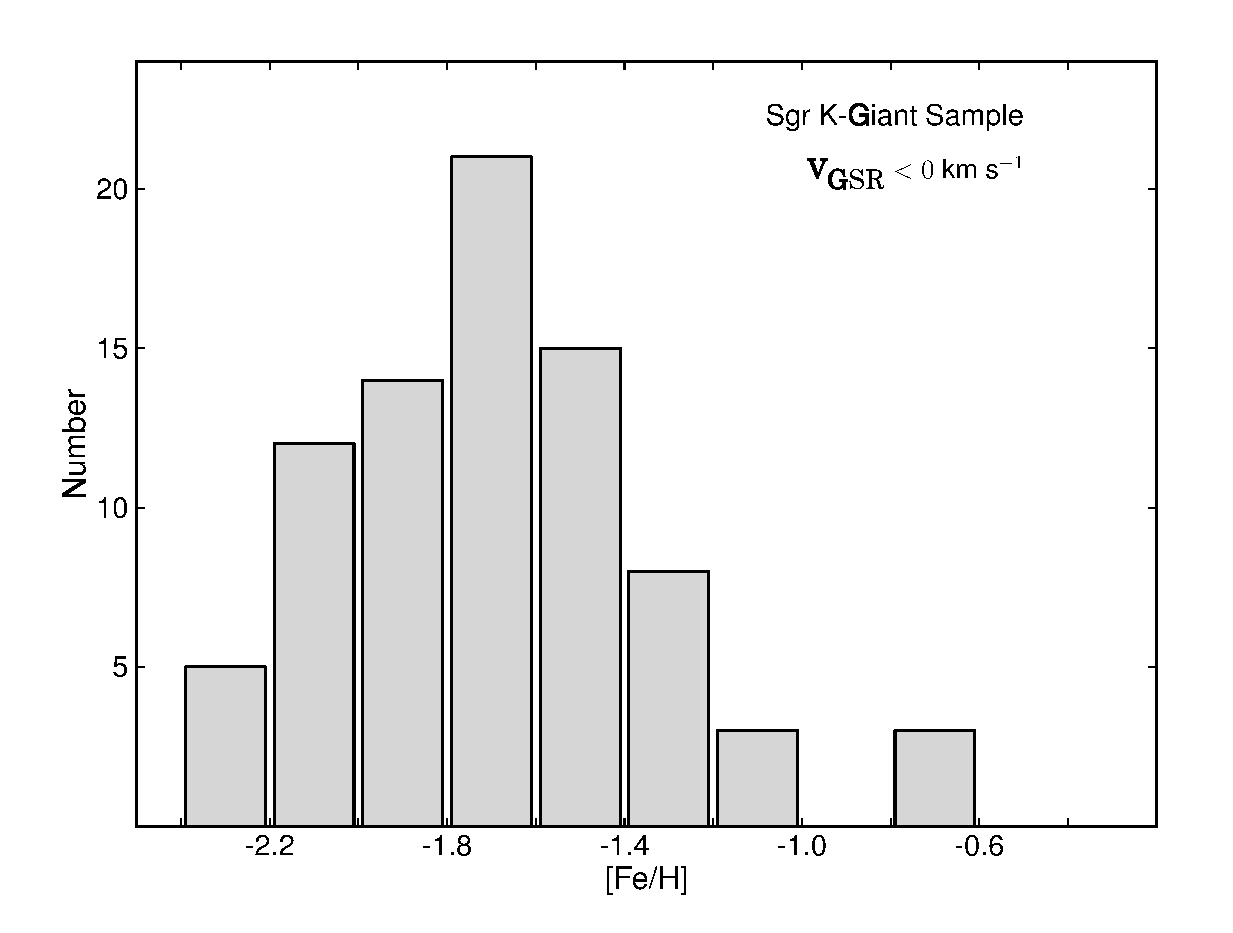
\includegraphics[width=\columnwidth]{./figures/fehhist.eps}
		\caption{Metallicity histograms for K-giant members in our negative galactocentric velocity sample, which is largely populated by Sgr debris from the Northern leading arm.}
		\label{fig:sgr-metallicity-hist}
	\end{figure}

	It is likely that our observed K-giant sample is biased towards more metal-poor members. Given a typical distance of $r_\odot\sim 40$ kpc for the Sgr debris in this region \citep{Belokurov;et-al_2006}, a 12 Gyr old Dartmouth \citep{Dotter;et-al_2008} isochrone with a metallicity of [Fe/H] $= -1.5$ falls directly within our target selection window. The more metal-rich isochrone with [Fe/H] $= -0.5$ does not pass through our selection range. This is consistent with our observed metallicities. Although this does not prohibit the possibility of more metal-rich members within our sample, it implies that our distribution may be slightly biased towards the metal-poor end of the MDF. The tail of our Sgr distribution extends from $-0.71$ to $-2.35$ dex.
\begin{comment}
	%However since only the oldest, and most metal-poor stars can form RR Lyrae stars, this is a biased sample. Investigating the age-metallicity relationship and the MDF for the Sgr debris requires an unbiased sample of metallicities. K-giants are an excellent stellar candidate for such measurements as all stars go through this evolutionary phase. Thus, their metallicities are more representative of the true MDF.
	% It does not fully represent the Sgr stream population, and we cannot infer information about the MDF of the stream from this sample. 
	%The metallicity distribution for our negative galactocentric sample is shown in Figure \ref{fig:sgr-metallicity-hist}. This illustrates a metal-poor population in Sagittarius, with a mean of $\langle$[Fe/H]$\rangle = -1.73\,\pm\,0.33$ dex. If we include only the stars attributed to Feature A (Sgr debris), this value is $\langle$[Fe/H]$\rangle = -1.69\,\pm\,0.36$. This value didn't change significantly (to $-0.68$ dex) when their less certain subsample was included, and the difference within samples is less than their intrinsic dispersion ($\sim 0.3$ dex). Although our sample size of K-giants is larger (47 in this bin) than the sample used by \citet{Chou;et-al_2007} (31 M-giants), their members were sparsely positioned, and covered larger spatial range of the Sgr debris. The tail of our distribution extends from $-0.71$ to $-2.35$ dex. %Admittedly even though we have a larger sample, it is insufficient to accurately represent the entire MDF for this region of the stream. 
	% In this Sgr sample, we cannot unequivocally state that \textit{every} star is a member of Sgr debris. It is likely we have some fraction of halo members present in our sample. When we consider the Sgr debris members (Feature A), the clump in velocities and metallicity space is significant. This clump was never reproduced in 10,000 Monte-Carlo simulations. Although we cannot exclude contamination in our sample by halo members, it is clear Sgr is the most influential population in our negative velocity sample \--- dominant in both kinematic and chemical space. As such, this sample demonstrates an unbiased representation of Sgr debris metallicities along the leading arm; one which shows a much greater metal deficiency than previously reported.
	
	This work illustrates the presence of a RGB metal-poor population in the Sgr debris, despite our target selection being biased towards this conclusion. 
	It is unlikely that the reported abundance gradients 
	
	
	either: 1 we're biased the other way and m-giants biased towards metal-rich and there is more work to be done, demonstrating the Sgr debris has an extremely large range of metallicities
	
		2. there is a larger abundance gradient larger than reported.
		
		
	
	As members of metal-rich members of Sgr 
	
	Since members of Sgr are identified in this region with muc 

	\subsubsection{Are the peaks at $-44$ and $-81$ km s$^{-1}$ in Feature A related?}
	\label{sec:sgr-peak-analysis}

	Two of our strongest observed features occur at $V_{GSR} = - 44$ and $-81$ km s$^{-1}$ (Figure \ref{fig:velocity-histogram}). This section examines whether these two peaks are observations of unique structures within the Sgr stream, or a sampling artefact of a single feature. \citet{Vivas;et-al_2008} noted that the most populated group in their sample of BHB and RR Lyrae stars had a mean velocity of $V_{GSR} = -49$ km s$^{-1}$ with a standard deviation of 22 km s$^{-1}$, some of which were from the  \citet{Sirko;et-al_2004} sample. Metallicity measurements of their variables returned a mean metallicity of $\langle$[Fe/H]$\rangle$ = $-1.72$ dex with a standard deviation of 0.28 dex. Our K-giant metallicities agree with these findings. In the equivalent bin ($-80 < V_{GSR} < -10$ km s$^{-1}$) we find a mean of $\langle$[Fe/H]$\rangle = -1.7$ dex and a standard deviation of 0.3 dex.  

%This sample comprised of nine RR Lyrae stars and five BHB stars from the $-80 < V_{GSR} < -10$ km s$^{-1}$
%In this region of high negative velocity, \citet{Vivas;et-al_2008} expect relatively high contamination from unrelated halo stars and suggest this may skew their kinematics. However they state this does not account for the diffuse metallicity distribution. The spread is likely representative of the true population, and not caused by the contamination of non-members into an otherwise narrow distribution. 
	
	\begin{figure*}[t!]
		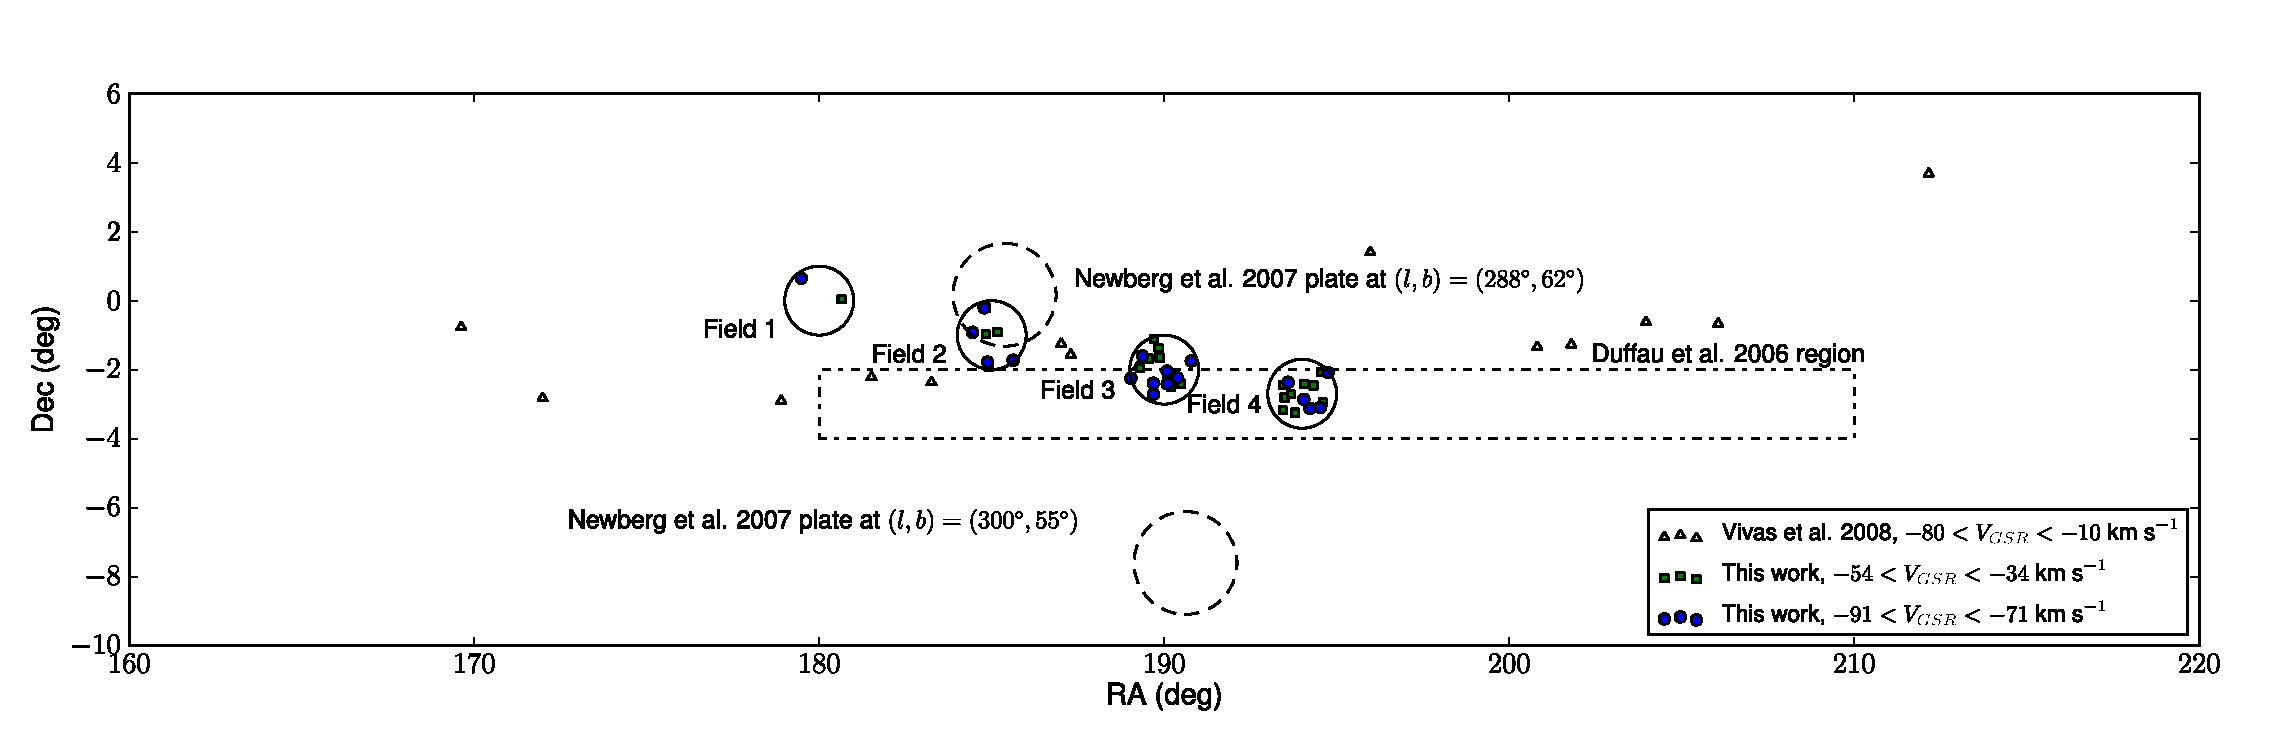
\includegraphics[width=\textwidth]{./figures/vivas-newberg-duffau.eps}
		\caption{The sky coverage examined in this data set which contains K-giants within our velocity bin ranges $-54 < V_{GSR} < -34$ km s$^{-1}$ (green squares) and $-91 < V_{GSR} < -71$ km s$^{-1}$ (blue circles), and the spatial coverage examined by \citet{Newberg;et-al_2007} who separately noted an identical peak at $V_{GSR} = -76$ km s$^{-1}$. The exact positions of stars found within this bin were unavailable. Sky covered by \citet{Vivas;et-al_2008} extends outside this plot, although all stars assigned to their peak at $V_{GSR} = -49$ km s$^{-1}$ are shown.}
		\label{fig:newberg-duffau-vivas-spatial}
	\end{figure*}

% However, contrary to \citet{Vivas;et-al_2008}, we find a narrow peak in this distribution whereas \citet{Vivas;et-al_2008} found a sparse distribution at [Fe/H] $\sim-1.7$ and no indications of contamination by non-members. Multiple groups have noted the peak near $V_{GSR} = -81$ km s$^{-1}$. 			

\citet{Vivas;et-al_2008} did not identify an additional peak at $-81$ km s$^{-1}$, whereas \citet{Duffau;et-al_2006} noted slight peaks at $-49$ and $-76$ km s$^{-1}$ in their sample which included 10 BHBs from the \citet{Sirko;et-al_2004} sample as well. The peak at $V_{gsr} = -76$ km s$^{-1}$ was also noted by \citet{Brink;et-al_2010} in their narrow spatial area (within our Field 2). Due to different galactocentric transformations, \citet{Brink;et-al_2010} measurements are offset from ours by up to $\sim{}+12$ km s$^{-1}$. 

\citet{Newberg;et-al_2007} found a 3-$\sigma$ excess of F-type stars in the $-80 < V_{GSR} < -48$ km s$^{-1}$ bin, centered on $-76$ km s$^{-1}$. Using the same galactocentric transformations as \citet{Newberg;et-al_2007}, our velocities would be consistently more positive with a mean offset of $+7.8\pm3.2$ km s$^{-1}$, implying our K-giants and these F-types are members of the same structure. 

%Distance estimates suggest this structure and the $-44/-49$ km s$^{-1}$ feature are distinct, although there are large uncertainties. RR Lyrae measurements place the \citet{Vivas;et-al_2008} feature at $7.5 < D < 9.5$ kpc and conservative estimates ($M_{g_0}=+4.2$) place the F-type sample at $11 \lesssim D \lesssim 14$ kpc


%\citet{Vivas;et-al_2008} argues that given the observational uncertainties, the \citet{Newberg;et-al_2007} stars may be members of their $-49$ km s$^{-1}$ structure, however the distances have not been reconciled yet. RR Lyraes in the \citet{Vivas;et-al_2008} $-49$ km s$^{-1}$ sample have a distance of $7.5 < D < 9.5$ kpc, whereas conservative estimates place the \citet{Newberg;et-al_2007} F-type sample at $11 \lesssim D \lesssim 14$ kpc. 
	

%This variation is spatially dependent, and as such the discrepancy between our peaks cannot be accounted for without tabulated spatial and kinematic information for each star. Mismatching the offsets could incur an incorrect variation of up to 11 km s$^{-1}$, simply because of the sky covered. 
%The discrepancy between our $-81$ km s$^{-1}$ peak and the $-76$ km s$^{-1}$ signature found by \citet{Newberg;et-al_2007} may be reconcilable. Using the same kinematic transformation as \citet{Newberg;et-al_2007}, our reported velocities would be consistently more positive with a mean offset of $+7.8\pm3.2$ km s$^{-1}$. \citet{Newberg;et-al_2007} notes that their $-76$ km s$^{-1}$ feature is more pronounced in the fainter $(l, b) = (300^\circ, 55^\circ)$ field, although upon recognising the feature they note it is also seen in their more northerly plate at $(288^\circ, 62^\circ)$. The more spatially prominent region covered by \citet{Newberg;et-al_2007} was not observed by \citet{Vivas;et-al_2008}, so the spatial overlap between these authors could not be fully investigated. 
	
%The sky covered by \citet{Duffau;et-al_2006} (which included the $-49$ and $-76$ km s$^{-1}$ features) ranged from ($\alpha, \delta$) $\approx$ (175 to 200$^\circ$, $-2$ to 0$^\circ$), which overlaps with this work and the \citet{Newberg;et-al_2007} fields (Figure \ref{fig:newberg-duffau-vivas-spatial}). Our $-81$ km s$^{-1}$ group is most spatially concentrated within ($\alpha, \delta$) = (189 to 195$^\circ$, $-3.5$ to $-1.5^\circ$), which overlaps where \citet{Duffau;et-al_2006} observed a similar peak and extremely close to the centroid where \citet{Newberg;et-al_2007} found their $-76$ km s$^{-1}$ peak of F-type stars. 

	\begin{figure}[h]
		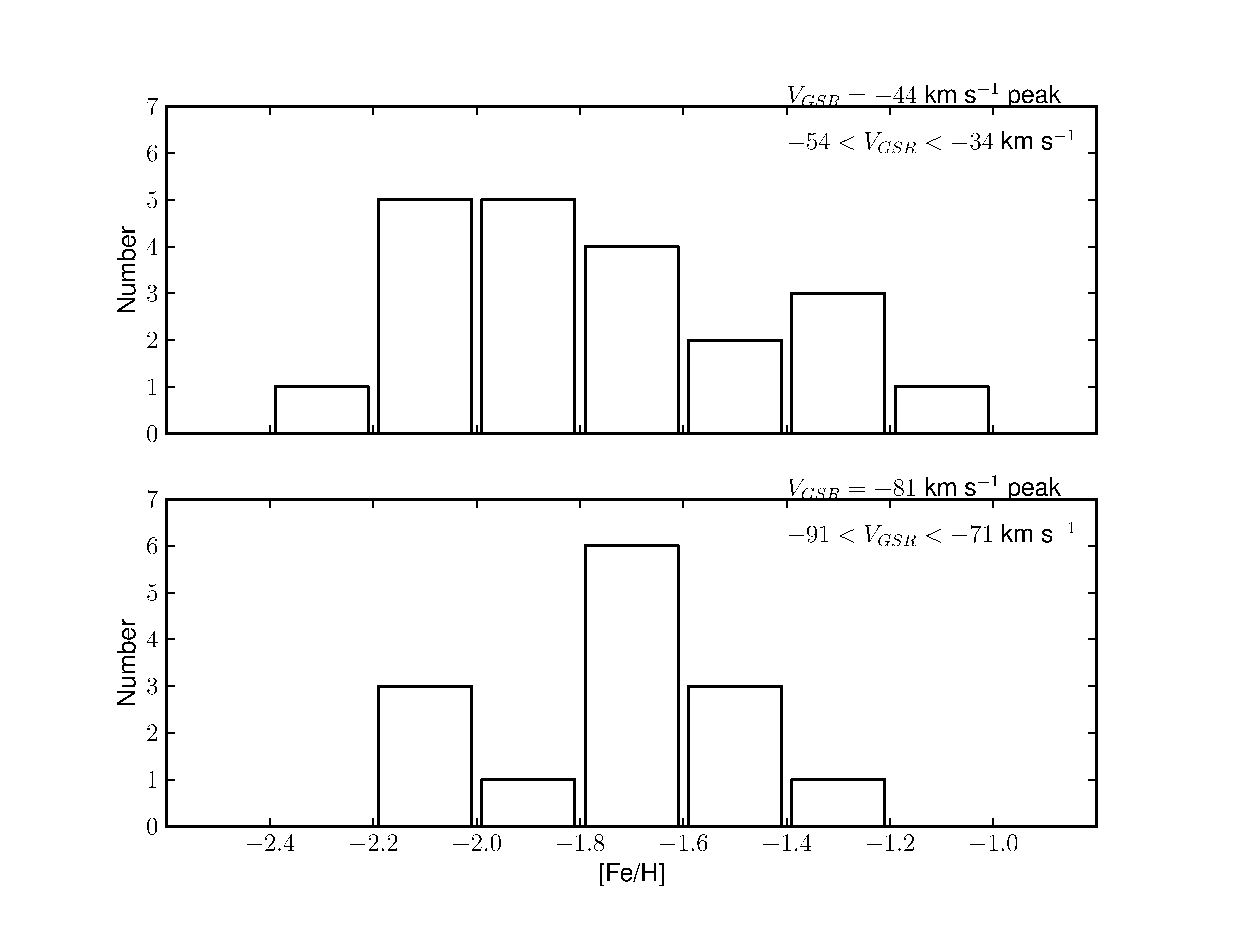
\includegraphics[width=\columnwidth]{./figures/feh-peak-bins.eps}
		\caption{Metallicity distribution for K-giants within the two nearby peaks at $V_{GSR} = -44$ km s$^{-1}$ (top) and $-81$ km s$^{-1}$ (bottom).}
		\label{fig:feh-peak-bins}
	\end{figure}

	The kinematic peaks near $V_{GSR} = -44$ and $-81$ km s$^{-1}$ overlap spatially (Figure \ref{fig:newberg-duffau-vivas-spatial}) and have been reported separately by multiple authors. Metallicities for these kinematic bins (Figure \ref{fig:feh-peak-bins}) do not demonstrate a substantial difference in mean abundance. If these two kinematic peaks are indeed separate 
	
	\citet{Vivas;et-al_2008} argue that given the observational uncertainties the \citet{Newberg;et-al_2007} sample at $-76$ km s$^{-1}$ may be members of their $-49$ km s$^{-1}$ sample. However the kinematic dispersions for these groups are quite low; 22 km s$^{-1}$ for the \citet{Vivas;et-al_2008} $-49$ km s$^{-1}$ sample and a mere 10 km s$^{-1}$ for the \citet{Newberg;et-al_2007} $-76$ km s$^{-1}$ sample. Moreover, the two peaks (within galactocentric transformation discrepancies) have been identified by many groups \citep[and this work]{Sirko;et-al_2004,Duffau;et-al_2006, Newberg;et-al_2007, Vivas;et-al_2008}. Separate repeat kinematic observations suggests these two features are distinct, although metallicity estimates from these observations do not demonstrate a mean abundance difference. Further abundance analysis may reveal a discernible difference between the two kinematic bins.
	
	%The two samples may have identifiable abundance discrepancies which could differentiate them.
	
	 %illustrates the metallicities for these two peaks. Although the sample size here is small, the $-81$ km s$^{-1}$ signature seems to peak in metallicity at the same point as our Sgr debris, whereas the $-44$ km s$^{-1}$ apex shows a sparse distribution.
	
	%A larger sample is favourable as it is problematic to distinguish or otherwise assign common membership to these moving groups.
	
	 %However due to larger spectroscopic sample obtained here, and previously repeated measurements by multiple authors, it is suggested these may be separate kinematic structures superimposed on one another. This claim is further strengthened given the kinematic dispersions from previous groups; 22 km s$^{-1}$ for the $-49$ km s$^{-1}$ by  \citet{Vivas;et-al_2008} and 10 km s$^{-1}$ for the $-76$ km s$^{-1}$ group by \citet{Newberg;et-al_2007}. If these structures are distinct, whether they are all associated to Sgr debris is a secondary question. Further investigation in this region is required.	
			
\end{comment}
	\subsection{Feature B \--- The Virgo Stellar Stream}
	\label{sec:the-vss}
	
	Another substructure which was distinguished from the general over-density of the VOD is the Virgo Stellar Stream \citep{Duffau;et-al_2006}. Several RR Lyrae stars were noted with a common velocity of $V_{GSR} = 130$ km s$^{-1}$ \citep{Newberg;et-al_2007, Prior;et-al_2009a}. \citet{Prior;et-al_2009a} also calculated metallicities of stars with this kinematic signature and found a mean [Fe/H] $= -1.95\,\pm\,0.1$ for the VSS, although this is based on RR Lyraes and is therefore potentially biased to the metallicity of the oldest populations. The RR Lyrae sample from \citet{Duffau;et-al_2006} found a $\langle$[Fe/H]$\rangle = -1.86$ with a much larger abundance spread of $\sigma = 0.40$, which was several times the relative uncertainty in individual values ($\sigma_{\mbox{[Fe/H]}} = 0.08$ dex). This led \citet{Duffau;et-al_2006} to infer the progenitor of the VSS was likely a dSph galaxy, as a large dispersion in $\mbox{[m/H]}$ indicates self-enrichment and implies the structure is a galaxy and not an isolated stellar cluster. We  also see an abundance spread within this kinematic bin, including some giants with kinematics and metallicities ($V_{GSR} = 130 \pm 9$ km s$^{-1}$, [Fe/H] =$ -2.0 \pm 0.16$) matching those found by \citet{Prior;et-al_2009a}. Monte-Carlo simulations reproduced these few targets a mere $\sim1$\% in 10,000 simulations \--- demonstrating their significance.
	
	%Based on measurements of seven type ab RRLs that have values of Vgsr that are consistent with membership, the VSS has <[FE/H]> = -1.86 and sigma= 0.40. Because this dispersion is several times the average of the sigma feh values (0.08) we conclude that the VSS has a significant range in [Fe/H]. A range of this magnitude is characteristic of all the dSph satellite galaxies of the Milky Way but not of the vast majority of globular clusters
	
	%We cannot unequivocally state whether members of the VSS are present in our K-giant sample \textit{only} from looking at kinematic signatures alone. In Figure \ref{fig:velocity-histogram} there is a peak at $V_{GSR} = +130$ km s$^{-1}$, however this is not as dominant as found by other authors.
	
	
	% The most likely VSS K-giant members are visibly separated from the bulk sample in velocity-metallicity space (Figure \ref{fig:velocity-metallicity}. Galactocentric velocities of these candidates ranges from $V_{GSR} = 127$ to $132$ km s$^{-1}$; which matches the kinematic signature seen by others studying the VSS. Furthermore the metallicities of our most probable candidates range from [Fe/H] = -1.89 to -2.03, identical to metallicity measurements of the VSS found by \citet{Prior;et-al_2009a} using RR Lyraes. Although RR Lyraes are typically representative of an older, more metal-poor population, it is interesting that these candidates match the VSS characteristics in spatial position, velocity, and metallicity. Monte-Carlo simulations replicated this clump at $V_{GSR} = +130$ km s$^{-1}$ and [Fe/H]$ = -1.95$ a mere 11 times in 10,000 \--- demonstrating their significance.
	
	%\begin{figure}[h]
	%	\includegraphics[width=\columnwidth]{./figures/vss-candidates_copy.eps}
	%	\caption{Galactocentric velocities and metallicity measurements for K-giants in our sample. Members contributing to the VSS peak are shaded, and our most probable VSS K-giant candidates are identified.}
	%	\label{fig:velocity-metallicity}
	%\end{figure}

	High resolution follow-up spectroscopy on these targets and other VSS candidates at higher metallicities in this kinematic range will provide crucial information about the origin of the VSS.  Investigating [$\alpha$/Fe] ratios in these candidates can constrain the mass of the VSS progenitor and discern whether the host was a dSph \citep{Venn;et-al_2004, Casetti-Dinescu;et-al_2009}.  Future observations are planned.

%K-Giants are the perfect candidate for high resolution spectroscopy, as they are cool enough to provide detailed elemental abundances, from which the formation history of the parent origin can be inferred.

	\subsection{Feature C \--- Sagittarius debris?}
	\label{sec:feature-c}

	The last significant kinematic substructure we identify in our data is Feature C. There are two peaks identified here at $V_{GSR} = 200$ and $240$ km s$^{-1}$. These features cannot be explained by a smooth halo distribution. \citet{Newberg;et-al_2007} identified a 4-$\sigma$ peak at $V_{GSR} = 200$ km s$^{-1}$ in their sample of F turnoff stars centered on $(l, b) = (288^\circ, 62^\circ)$. Our nearest field to their plate (Field B) hosts only one star associated with this peak; most of our these stars are located within our most populated Field D. \citet{Prior;et-al_2009b} also noted stars in this kinematic range and compiled a list of authors who have also observed such peaks (see \citet{Sirko;et-al_2004, Duffau;et-al_2006, Starkenburg;et-al_2009}). \citet{Prior;et-al_2009b} argue these stars may be associated with trailing debris of Sagittarius, as suggested by models (LJM05, LM10).  Although this trailing debris would be much closer than the nearby visible leading arm, these observations support the interpretation by \citet{Prior;et-al_2009b} as the metallicities are quite similar to the nearby Sgr debris.
	
%In any case we can be sure that the CaT-[Fe/H] calibration yields realistic metallicities. 
 
	This substructure has a range of metallicities on our scale. These metallicities were derived with the distance modulus to the VOD/VSS, and may not be exact representations. As such the abundance dispersion we observe is either representative, or these stars have a common metallicity and are dispersed along the line of sight. Unfortunately neither can be positively excluded without further observations. If these peaks are associated with the trailing debris of Sagittarius debris, they are likely to be further away than the VOD. On our scale that would make these stars more metal-rich than shown in Figure \ref{fig:monte-carlo}. However the nearest trailing debris particles predicted from any best-fitting dark halo potential that could explain this kinematic peak occurs at $\sim\Lambda_\odot = 310^\circ$; our observations range in $\Lambda_\odot$ between $256^\circ-273^\circ$. Whether this substructure is separate from Sagittarius debris or not remains equivocal.	
	

\section{Carbon Stars}
	
	In our sample we have identified five carbon stars. With the colour selections to target K-giants, this region also overlaps with where we would expect to find carbon stars (Figure \ref{fig:carbon-sdss}). Although these stars were not specifically targeted, their surface densities are so low \citep[$\approx$ 1 per 50 deg$^2$;][]{Green;et-al_1994} that we would not expect them as a substantial contaminant.  Although our sky coverage is small ($\sim$12.5 deg$^2$), the observed carbon star spatial density is $\sim20$x higher than expected. All five carbon stars are recognisable by the presence of distinctive 4737- and 5165 \AA\, Swan C$_2$ bands.

\begin{comment}
	\begin{figure}[h]
		\includegraphics[width=\columnwidth]{./figures/carbon_copy.eps}
		\caption{J-H and H-K colours for carbon stars recovered by \citet{Totten;et-al_2000}, and those found in this sample. Four of our five carbon stars are represented with plus symbols (+); 2MASS photometry for our faintest carbon star was not available. Carbon stars identified in this work have been shaded for clarity. This plot is an adaptation of Figure 3 in \citet{Totten;et-al_2000}.}
		\label{fig:carbon-colours}
	\end{figure}
\end{comment}
		
\begin{figure}[h!]
	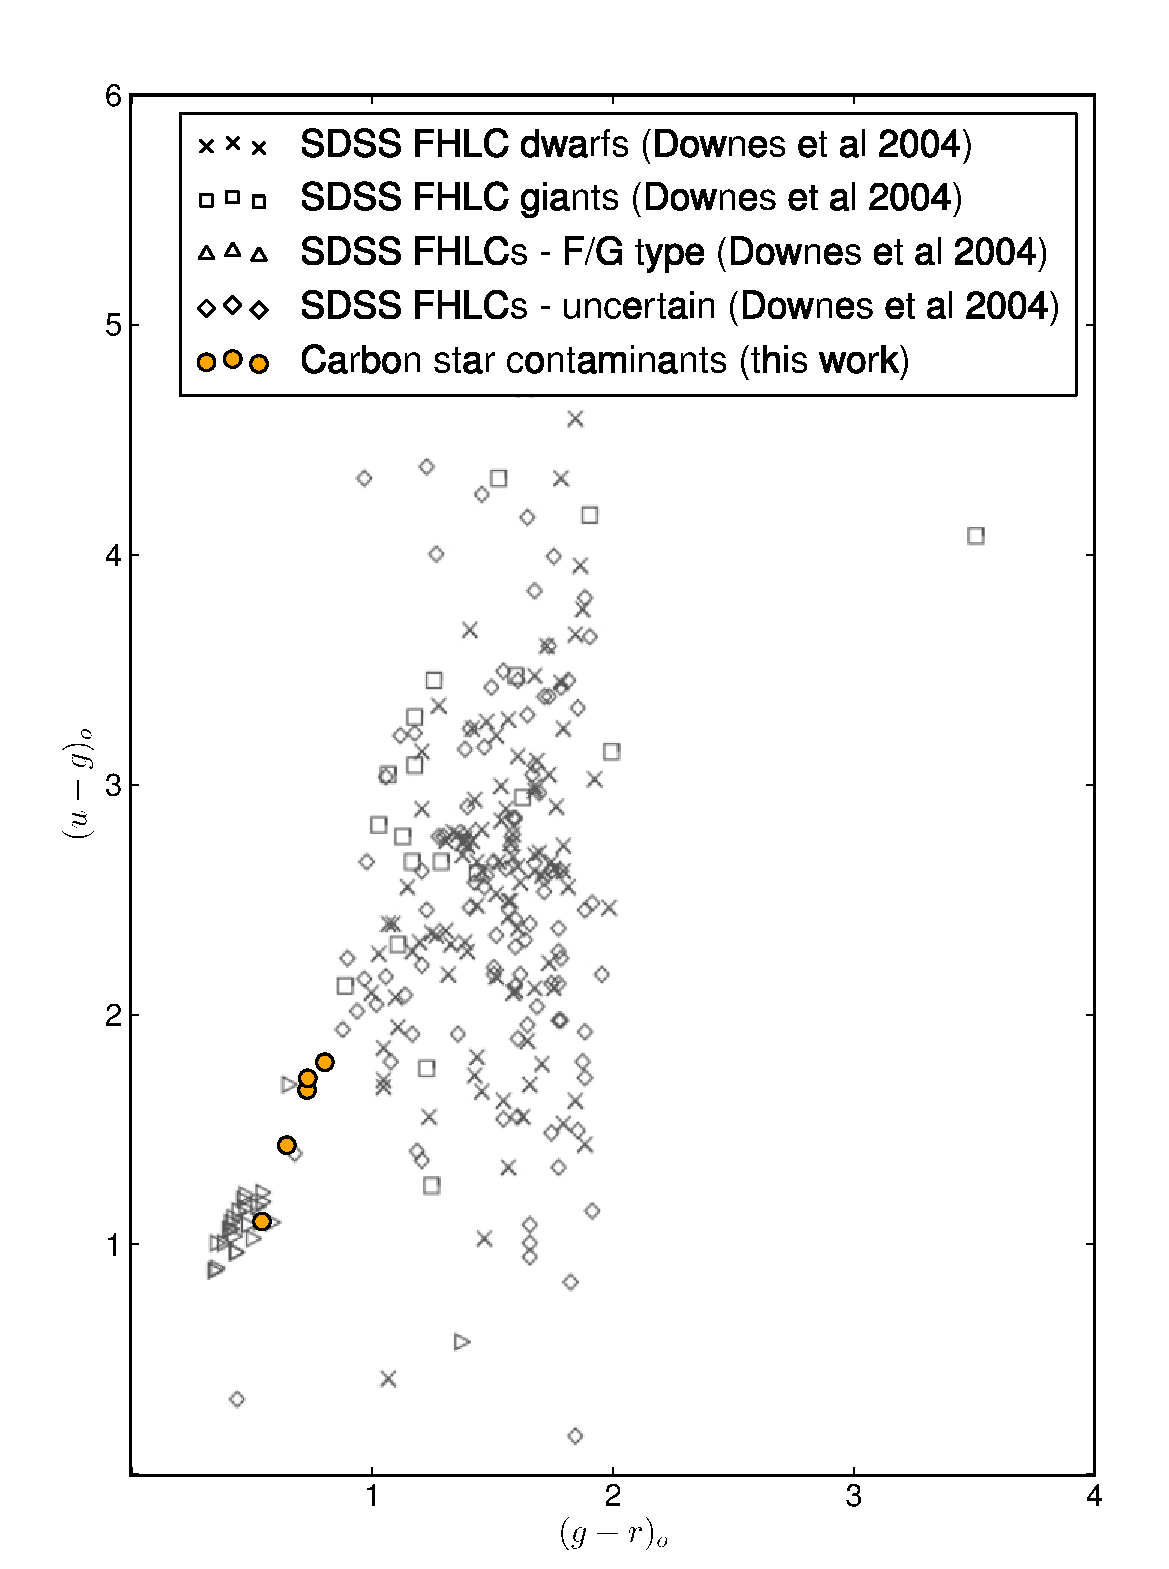
\includegraphics[width=\columnwidth]{./figures/carbonstarcolor.eps}
	\caption{Sloan \textit{u \--- g} and \textit{g \--- r} colours for our carbon stars, and the identified carbon stars and classifications by \citet{Downes;et-al_2004}. Carbon stars identified in this work have been shaded for clarity.}
	\label{fig:carbon-sdss}
\end{figure}

	%There are at least three kinds of carbon stars present in the halo; (i) N-type carbon stars, (ii) giant CH-type carbon stars and (iii) and dwarf CH-type carbon stars \citep{Totten;Irwin_1998}. N-type carbon stars are formed by carbon-enriched dredge-up during the post-main-sequence phase of a normal asymptotic giant branch (AGB) star. First generation carbon stars (CH-type) are not considered to have undergone carbon-enriched dredge-up, and their carbon abundance is attributable to mass transfer within a binary system.

%These dwarf carbon stars are believed to form in binary systems where material has accreted from a now-invisible companion during its ascent up to the AGB \citep{Dahn;et-al_1977}. Giant CH-type carbon stars are similar to metal-poor carbon stars found in globular clusters \citep{Harding_1962} and in some dSph galaxies \citep{Demers;Battinelli_2002}. 	

	 Dwarf carbon stars exhibit a spectral signature which mimics that of a typical CH-type giant carbon star, however they have anomalous JHK colours \citep{Green;et-al_1992} and high proper motions. The existence of the 4300 \AA{} CH G-band is representative of a CH-type carbon star, and is found in all five of our carbon stars. SDSS photometry for our stars match well with the F/G-type CH carbon stars identified by \citet{Downes;et-al_2004}, as seen in Figure \ref{fig:carbon-sdss}. However these targets were not spectroscopically observed in the SDSS follow-up survey SEGUE. Additionally, through comparisons with previous carbon-type star catalogues \citep{Totten;Irwin_1998, Downes;et-al_2004, Goswami;et-al_2010}, the stars tabulated in Table \ref{tb:carbon-stars} are previously unclassified carbon stars. This is largely because our objects are too faint to have been observed by previous spectroscopic carbon star surveys.
	
\begin{deluxetable}{cccccccccccc}
\tablewidth{0pt}
\tabletypesize{\scriptsize}
\tablecaption{Properties of carbon stars found in our sample \label{tb:carbon-stars}}
\tablehead{
	\colhead{SDSS Name J+\tablenotemark{a}} & 
	\colhead{$M_g$} &
	\colhead{\it{u-g}} &
	\colhead{\it{g-r}} &
	\colhead{\it{r-i}} &
	\colhead{\it{i-z}} &
	\colhead{\it{H-K}} &
	\colhead{\it{J-H}} &
	\colhead{$\mu_{\alpha\cos{\delta}}\tablenotemark{c}$} &
	\colhead{$\mu_\delta\tablenotemark{c}$} &
	\colhead{$V_{GSR}$} & 
	\colhead{Likely} \\
	& & & & & & & & (mas yr$^{-1}$) & (mas yr$^{-1}$) & (km s$^{-1}$) & dwarf?
} 

\startdata
121740.94-001839.5 & 18.66 & 1.10 & 0.54 & 0.16 & 0.05 & ...\tablenotemark{b}& ...\tablenotemark{b} & \phn$-3.0 \pm 5.4$  & $-18.0 \pm 5.4$\phn & $\phn-71 \pm 34$ & Yes\\
121853.18-004628.4 & 17.71 & 1.67 & 0.73 & 0.22 & 0.11 & \phd0.24 & 0.36 &  \phn$-3.7 \pm 4.5$ & $-0.5 \pm 4.5$ & $+176 \pm 9$ & - \\
122053.71-011709.5 & 17.65 & 1.79 & 0.80 & 0.26 & 0.13 & \phd0.16 & 0.56 &  \phn$-7.3 \pm 4.3$ & $-3.9 \pm 4.3$ & $\phn+31 \pm 11$ & - \\
125410.80-032744.0 & 18.59 & 1.43 & 0.64 & 0.22 & 0.05 & \phd0.56 & 0.32 &$-21.1 \pm 5.0 $ & $-7.7 \pm 5.0$ & $\phn-41 \pm 9\phn$ & Yes \\ 
125416.52-031437.6 & 16.85 & 1.72 & 0.73 & 0.25 & 0.11 & -0.11 & 0.50 & $-19.8 \pm 4.2$ & \phd\phn$8.7 \pm 4.2$& $\phn+15 \pm 4\phn$ & Yes \\
\enddata
\tablenotetext{a}{To keep with convention, positional information has been truncated. Full information available through the SDSS archive.}
\tablenotetext{b}{No \textit{JHK} photometry is available for this object as it is fainter than the 2MASS survey limit.}
\tablenotetext{c}{Proper motions taken from the PPMXL Catalog \citep{Roser;et-al_2010}.}
\end{deluxetable}

	There is 2MASS photometry available for four of these stars. Of those, two stars (SDSS J125410.80-032744.0 and J125416.52-031437.6) exhibit anomalous JHK colours and significant ($> 3\sigma$) proper motions; characteristics of a dwarf carbon star. A third star also exhibits significant proper motion (SDSS J121740.94-001839.5), however JHK photometry is unavailable. The two remaining stars in our sample have JHK photometry characteristic of the F/G type CH carbon stars found by \citet{Downes;et-al_2004} in their Faint High-Latitude Carbon (FHLC) star survey (Figure \ref{fig:carbon-sdss}), and do not exhibit significant proper motion - which strongly suggests they are not dwarfs \citep{Green;et-al_1994, Deutsch_1994}. All identified K-giant stars in our distilled sample had no proper motion detectable above measurement errors.  These carbon star kinematics are representative of a typical halo population.

	
\section{Conclusions}
\label{sec:conclusions}

%Measuring the gravity sensitive Mg I triplet lines in both synthetic and observed spectra, we have demonstrated an excellent dwarf/giant separation criterion.
	We present spectroscopic observations of K-type stars in a crowded region of the 'Field of Streams', where significant substructure is present. We utilise the gravity-sensitive Mg I triplet to separate giants and dwarfs. Radial velocities and metallicities of 178 K-giants have been determined. We have recovered kinematic substructure found by other authors, which cannot be explained by a smooth halo distribution. Highly negative velocity signatures match those expected by the Sagittarius stream debris, and we identify a clump of K-giants with metallicities and kinematics which make them highly probable members of the Virgo Stellar Stream.

	%Through investigating Sgr debris we have identified multiple kinematic peaks as found by other authors. These peaks have a small kinematic separation compared to the observational uncertainties. Although our sample size is small, the first hint of these structures as being separate entities has been identified through apparent discrepancies in their metallicity distribution functions. 
	Stars in this region of the Sagittarius stream are kinematically sensitive to the shape of the Galactic dark halo. As such, we have compared our velocity distribution to the Sgr-Milky Way dark matter models of \citet{Law;et-al_2005, Law;Majewski_2010}. Typically, leading arm debris favour prolate models and trailing arm debris favour oblate models. A prolate dark halo predicts no debris in our observed fields. If the spheroid is prolate and LJM05 presents an accurate representation, we would not expect Sgr debris to dominate our sample (as it does so) even if we were $\Delta{}B_\odot\sim10^\circ$ closer to the great circle best-fit. However, Sgr debris is our most significant kinematic structure observed. No single model perfectly represents our data, although we find the more recent tri-axial model (LM10) best represents our observed kinematics. Future tri-axial models of Sgr with bifurcation treatment are likely to more closely represent our observations.
	
	Observed metallicities for K-giants in this region of the Sgr stream are notably lower than expected based on other Sgr samples, demonstrating the presence of a metal-poor population in the  Sagittarius debris. Although isochrones indicate we may be biased towards metal-poor members at these distances, these stars are unequivocally Sagittarius in origin. Metallicity gradients reported suggest a mean of $\langle[$Fe/H$]\rangle\sim{}-1.2$, whereas our population has $\langle[$Fe/H$]\rangle = -1.7 \pm 0.3$ dex. Previously reported metal-poor abundances in this region have been from old RR Lyraes where we would expect $\langle[$Fe/H$]\rangle\sim{}-1.7$ dex or young M-giants where $\langle[$Fe/H$]\rangle\sim{}-0.7$ dex is reasonable. Thus the sample presented here is more representative of the complete MDF. These observations also demonstrate that the Sagittarius stream hosts a substantially larger abundance range than previously found, including a previously uncovered metal-poor population of K-giants.
	
	
	%This suggests either higher abundance gradients along the stream than previously reported, or the Sgr debris has an extremely wide metallically spread. Although biased towards metal-rich members, \citet{Chou;et-al_2007} find a mean metallicity of $\langle[$Fe/H$]\rangle = -0.72 \pm 0.30$ dex along the leading arm from M-giants. These contrasting observations imply the metallicity distribution function of the debris remains largely unknown. 
\begin{comment}

	at one point Sagittarius hosted a substantial spread in abundances, and that the metallicity distribution function for the debris remains a mystery.
	
	including the metal-poor population found here.
		
	This suggests that thereAlthough this K-giant sample 	
	M-giant studies in this region by 
	
	These observations host a sample of K-giant metallicities for Sagittarius debris along the leading arm. 
	
	In contrast to   who found a mean metallicity of  stream in their metal-rich biased M-giant sample, we find a mean metallicity of  Although we have large uncertainties in our metallicity distribution, this is indicative of a more metal-poor population present within this region of the stream.%This is representative of the generally more metal-poor, older population along this region of the stream.
	
	This work illustrates the presence of a RGB metal-poor population in the Sgr debris, despite our target selection being biased towards this conclusion. 
	It is unlikely that the reported abundance gradients 
	
	
	either: 1 we're biased the other way and m-giants biased towards metal-rich and there is more work to be done, demonstrating the Sgr debris has an extremely large range of metallicities
	
		2. there is a larger abundance gradient larger than reported.
		
		
	
	As members of metal-rich members of Sgr 
	
	Since members of Sgr are identified in this region with muc 
\end{comment}

\section{Acknowledgements}
ARC acknowledges the financial support through the Australian Research Council Laureate Fellowship 0992131. SK and GDaC acknowledge the financial support from the Australian Research Council through Discovery Program DP0878137.

This publication makes use of data products from the Two Micron All Sky Survey, which is a joint project of the University of Massachusetts and the Infrared Processing and Analysis Center/California Institute of Technology, funded by the National Aeronautics and Space Administration and the National Science Foundation.

Funding for the SDSS and SDSS-II has been provided by the Alfred P. Sloan Foundation, the Participating Institutions, the National Science Foundation, the U.S. Department of Energy, the National Aeronautics and Space Administration, the Japanese Monbukagakusho, the Max Planck Society, and the Higher Education Funding Council for England. The SDSS Web Site is http://www.sdss.org/.

The SDSS is managed by the Astrophysical Research Consortium for the Participating Institutions. The Participating Institutions are the American Museum of Natural History, Astrophysical Institute Potsdam, University of Basel, University of Cambridge, Case Western Reserve University, University of Chicago, Drexel University, Fermilab, the Institute for Advanced Study, the Japan Participation Group, Johns Hopkins University, the Joint Institute for Nuclear Astrophysics, the Kavli Institute for Particle Astrophysics and Cosmology, the Korean Scientist Group, the Chinese Academy of Sciences (LAMOST), Los Alamos National Laboratory, the Max-Planck-Institute for Astronomy (MPIA), the Max-Planck-Institute for Astrophysics (MPA), New Mexico State University, Ohio State University, University of Pittsburgh, University of Portsmouth, Princeton University, the United States Naval Observatory, and the University of Washington.
\bibliographystyle{apj}
\bibliography{draft}
	
\end{document}


